\documentclass[a4paper]{article}
\usepackage[T1]{fontenc} % codifica del font 
\usepackage[utf8]{inputenc} % aggiunge le lettere accentate italiane
\usepackage[italian]{babel} % lingua del documento
\usepackage{tikz}
\usepackage{enumerate, enumitem}
\usepackage[top=1in, bottom=1.25in, left=0.55in, right=0.55in]{geometry}
\usepackage{graphicx}
\usepackage{tcolorbox}
\usepackage{tabularray}
\usepackage{hyperref}
\usepackage{listings}
\setlength\parindent{0pt}
\setlength\parskip{0.75em}
\usepackage{comment}

\author
{
		Miranda Pasquale \and Matricola: N86004643 \and
		Mennillo Vincenzo \and Matricola: N86004494
}
\title
{
	{\huge Università degli Studi di Napoli Federico II}\\
	\begin{center}
		
\includegraphics{res/uni_logo}
	\end{center}		
	
	Corso di Laurea Triennale in Informatica \\
	Anno Accademico 2023/2024 \\
	Insegnamenti:\\ \vspace{2 cm} 
	Basi di Dati e Sistemi Informativi I \hfill Object
	Orientation \\
	Professore \hfill Professore \\
	\textbf{Silvio Barra} \hfill \textbf{Porfirio Tramontana} \\
	\vspace{2 cm}
	\huge Traccia 3: Sistema Informativo Dei Calciatori
}

\newcommand{\pk}[1]{\underline{#1}}
\newcommand{\fk}[1]{#1$\uparrow$}
\newcommand{\pfk}[1]{\fk{\pk{#1}}}

\begin{document}

\maketitle
\newpage
\tableofcontents
\newpage

\section{Traccia 3}

\subsection{\Large Descrizione della Traccia}
\bigskip

Si sviluppi un sistema informativo, composto da una base
di dati relazionale e da un applicativo Java dotato
di GUI (Swing o JavaFX), per la gestione
di calciatori di tutto il mondo.

Ogni calciatore è caratterizzato da nome, cognome,
data di nascita, piede (sinistro, destro o ambidestro),
uno o più ruoli di gioco (portiere, difensore,
centrocampista, attaccante) e una serie
di feature caratteristiche (ad esempio colpo di testa,
tackle, rovesciata, etc.).

Il giocatore ha una carriera durante
la quale può militare in diverse squadre di calcio.
La militanza in una squadra è caratterizzata
da uno o più periodi di tempo nei quali
il giocatore era in quella squadra.
Ogni periodo di tempo ha una data di inizio
ed una data di fine.
Durante la militanza del giocatore nella squadra
si tiene conto del numero di partite giocate,
del numero di goal segnati e del numero
di goal subiti (applicabile solo ai giocatori
di ruolo portiere). Il giocatore può inoltre vincere
dei trofei, individuali o di squadra.

Il giocatore può avere anche una data di ritiro
a seguito della quale decide di non giocare più.
Le squadre di calcio sono specificate
dal loro nome e nazionalità.

L’amministratore del sistema si identifica con una login
ed una password e ha il diritto di inserire
nuovi giocatori nella base di dati, modificarne i dati,
aggiungere ulteriori informazioni
oppure eliminare un giocatore.

L’utente generico può vedere l’elenco dei giocatori e
le loro caratteristiche e può richiedere diverse ricerche,
ad esempio filtrando i giocatori per nome, per ruolo,
per piede, per numero di goal segnati,
per numero di goal subiti, per età,
per squadre di appartenenza.

Per gruppi da 3 persone: I giocatori dopo la fine
della carriera possono diventare allenatori o dirigenti.
Il sistema continua a mantenere una parte
delle informazioni (squadra, numero di partite
e trofei vinti) anche per allenatori e dirigenti.

Inoltre, può accedere al sistema anche un terzo tipo
di utente, consistente nel Giocatore stesso.
Egli ha una sua login e password e può modificare
unicamente i dati relativi a sé stesso.

\section{Database}

\subsection{Analisi dei Requisiti}

Nell'affrontare questo progetto abbiamo Nell'affrontare questo progetto abbiamo deciso - seguendo i suggerimenti dei Docenti -, di svolgere
la traccia proposta entro una cornice più ampia, preservando il ruolo centrale delle entità-calciatori,
ma ponendole al centro di un contesto più complesso, rappresentativo dell'intero mondo calcistico.

A questo scopo, abbiamo effettuato una serie di indagini e ricerche sui principali siti di informazione riguardanti il calcio. Segnatamente, ci siamo basati sulle informazioni reperibili da Wikipedia, siti ufficiali delle principali confederazioni calcistiche, Transfermarkt, Fantagazzetta, FootballManager e vari altri siti e giornali di argomento calcistico.

Con non poca difficoltà abbiamo cercato di astrarre quelle che, a una prima analisi, abbiamo giudicato essere le
caratteristiche fondamentali del sistema-calcio nel mondo reale e di configurarle, al meglio delle nostre
possibilità, nel progetto assegnatoci.

\bigskip
\bigskip

Un primo aspetto concettuale - che sin da subito è risultato evidente - è che il sistema-calcio è
gerarchico, strutturato come un vero e proprio governo e costituito da confederazioni internazionali,
federazioni nazionali e leghe calcistiche (es. FIFA, UEFA, COMBEBOL, FIGC, \dots), che definiscono
le regole del gioco, organizzano le varie competizioni e sono pertanto il fulcro dell'intero sistema.

Per semplicità, a partire da questo momento con il termine "confederazione" faremo
riferimento indistintamente a confederazioni, federazioni, leghe e a qualsiasi altro ente
organizzativo che svolga un ruolo attivo nella gestione della struttura del sistema-calcio.

Ogni confederazione calcistica è associata con uno ed un solo paese.
\newline
Come per le confederazioni, trasporremo su di un livello di astrazione superiore anche il concetto di paese.
Identificheremo come "paese" i concetti di regione, nazione, continente e persino il mondo intero.

Data la relazione che intercorre tra un paese ed una confederazione calcistica, queste ultime
potranno essere suddivise in tre grandi categorie:

\begin{itemize}
	\item Confederazioni nazionali;
	\item Confederazioni continentali;
	\item Confederazioni mondiali.
\end{itemize}

Sottolineiamo che tale suddivisione opera una certa semplificazione, in quanto
esistono confederazioni subcontinentali, confederazioni regionali e così via; ci è sembrato
superfluo elevare ulteriormente la granularità della nostra analisi.

Un'ulteriore aspetto concettuale che abbiamo rilevato in corso di ricerca è che -
come già accennato - le confederazioni sono organizzate in ordine gerarchico: le confederazioni
nazionali fanno parte di confederazioni continentali, che a loro volta sono
membri di confederazioni mondiali (es. la FIGC è membro della UEFA che a sua volta è membro
della FIFA).
Questo pattern si ripresenta per la quasi totalità delle confederazioni che abbiamo osservato:
le uniche e rare eccezioni fanno capo a confederazioni minori isolate, esterne alla FIFA,
che quindi non sono in associazione con nessun'altra confederazione.
Dalle ricerche effettuate abbiamo notato che a tutti gli effetti il sistema-calcio fa capo
alla FIFA e pertanto si è deciso di escludere il calcio esterno alla FIFA.


È indiscutibile che il concetto di confederazione calcistica, insieme a quello di paese,
formino la base sulla quale poggia tutta l'organizzazione calcistica mondiale.

\bigskip
\bigskip

Come detto in precedenza, ciascuna confederazione organizza diverse competizioni calcistiche.
Una competizione calcistica può essere analizzata secondo diversi criteri;
se consideriamo come elemento discriminante il tipo di squadra che può parteciparvi, è possibile
dividere le competizioni calcistiche in due categorie:
\begin{itemize}
	\item Competizioni per squadre di tipo club;
	\item Competizioni per squadre di tipo nazionale.
\end{itemize}

Tuttavia, se l'elemento discriminante è il format che caratterizza una competizione
calcistica, queste possono essere raggruppate in tre categorie:
\begin{itemize}
	\item Competizioni di tipo campionato;
	\item Competizioni di tipo torneo;
	\item Competizioni di tipo supercoppa.
\end{itemize}

In effetti, l'analisi delle competizioni calcistiche è ben più complessa di quella che stiamo descrivendo. Infatti, una competizione può svolgersi anche secondo una formula (girone all'italiana, eliminazione diretta, \dots),
che può variare in base all'edizione della competizione che si sta considerando,
e secondo cui può variare anche il numero di partecipanti. Risulta pertanto estremamente complicato astrarre coerentemente questo insieme di informazioni.

Nonostante le difficoltà, abbiamo cercato di conciliare e preservare entrambi i punti di vista sulle
competizioni calcistiche e, seguendo la traccia, abbiamo selezionato come preminente uno
dei due.

Nella traccia si fa un chiaro riferimento alle squadre di calcio, e pertanto ci è sembrato
più corretto prediligere la prospettiva che mettesse maggiormente in risalto questo aspetto;
pertanto, dati i nostri scopi, il concetto di competizione calcistica sarà in primo luogo
considerato in base al tipo di squadra che può parteciparvi, e solo in secondo luogo
in base al tipo di format.

Vale la pena fare un'importante precisazione: una confederazione nazionale non potrà organizzare competizioni
calcistiche per squadre di tipo nazionale.

\bigskip
\bigskip

Come ben noto, ogni competizione ha diverse edizioni, ciascuna delle quali si svolge entro
una specifica stagione calcistica.

Dalle ricerche effettuate è emerso che, nell'ambito di un'unica confederazione organizzativa e di uno specifico format, è possibile classificare le edizioni competitive per gradi di importanza (es. nella FIGC la serie A è il campionato di "primo
livello", la serie B il campionato di "secondo livello").

Abbiamo concluso che non può esistere una squadra di calcio che, nella
stessa stagione, partecipi a due diverse competizioni dello stesso format orgnizzate dalla stessa
confederazione.

Una stagione calcistica è a tutti gli effetti l'unità di misura temporale del calcio. E' scandita in un periodo che intercorre tra due anni consecutivi (es. Stagione 2023-2024).
Per le competizioni di squadre di tipo nazionale, il concetto di stagione calcistica
coincide con la durata di un anno solare (es. Stagione 2023-2023).

In una qualsiasi istanza di un'edizione competitiva, al termine delle competizioni previste, ad alcune squadre tra le partecipanti vengono assegnati dei trofei, in base alla loro posizione in classifica.

Un trofeo, quindi, risulta concettualmente associato a una specifica edizione di una competizione
calcistica; d'altra parte, le nostre ricerche hanno evidenziato la presenza di trofei calcistici
indipendenti dalle competizioni.


Pertanto, dal punto di vista astratto, si è reso necessario operare una distinzione tra i trofei calcistici
che saranno sempre correlati a delle competizioni, e premi calcistici che, invece
occorrono in maniera indipendente.

Un ultimo concetto chiave relativo al mondo del calcio è quello di "squadra di calcio".
Una squadra di calcio appartiene a una nazione e fa sempre parte della
confederazione della nazione a cui è associata.
Una squadra può far parte di due grandi categorie:
\begin{itemize}
	\item Squadra di calcio di tipo club;
	\item Squadra di calcio di tipo nazionale.
\end{itemize}

Dalle nostre ricerche è inoltre risultato che una squadra di calcio può partecipare
solo alle competizioni (del tipo di squadra corrispondente) organizzate dalla confederazione
di cui è membro o da confederazioni che contengono la confederazione calcistica di cui
è membro (es. la Salernitana, squadra di calcio di tipo club che appartiene alla FIGC,
può partecipare alle competizioni organizzate dalla FIGC, ma anche a quelle organizzate
dalla UEFA (Professore, la Salernitana in Europa è e rimarrà un sogno!),
ma non alle competizioni organizzate dalla COMBEBOL).

Un'ultima precisazione: abbiamo deciso di escludere dalla nostra trattazione sia il calcio
femminile che il calcio giovanile, non rappresentando questi un ampliamento efficace del presente progetto.
Aggiungeremo che, in ogni caso, sarebbe stato gestibile in modo essenzialmente identico, con la sola aggiunta di qualche attributo; è stato pertanto ritenuto uno sforzo inutile.

\bigskip
\bigskip

Questo è, in estrema sintesi, l'arricchimento che abbiamo deciso di conferire al nostro progetto.
Ricordiamo però che il principale scopo del nostro lavoro è costruire un sistema informativo
per la gestione di calciatori di tutto il mondo.

Le ricerche effettuate e le conclusioni a cui siamo giunti non rappresentano
un mero esercizio di stile, ma ci permetteranno di disporre di una descrizione più sofisticata dei singoli calciatori - a scapito della semplicità formale del progetto.

\bigskip
\bigskip

Ogni calciatore avrà una nazione di nascita, una o più nazionalità e,
come indicato da traccia, una carriera durante la quale può militare in diverse
squadre di calcio.

A questo proposito è doveroso fare una importante precisazione. Vista la natura più dettagliata
della nostra visione del progetto, anche il concetto di militanza di un calciatore in una squadra
di calcio sarà più dettagliato.

Il nostro concetto astratto di militanza sarà la presenza di un calciatore in una squadra
durante una stagione calcistica, visto che, come detto, la stagione è l'unità di misura
temporale del mondo calcio.

Abbiamo deciso quindi di non considerare la data di inizio e fine di una certa militanza in
quanto al nostro livello di dettaglio è impossibile da gestire in modo coerente e corretto,
mantenendo anche un certo livello di astrazione.
Infatti, a seguito delle nostre ricerche abbiamo notato che il regolamento vigente
prevede che un cambio di militanza di un calciatore da una squadra ad un'altra
possa avvenire solo in particolari periodi di tempo, detti "finestre di mercato",
che per altro sono variabili in base alla stagione considerata e alla confederazione
calcistica cui fanno riferimento; ecco il motivo per il quale non è possibile utilizzare
le date come richiesto da traccia.
Sarebbe, infatti, impossibile controllare correttamente le variazioni della militanza di un calciatore
durante la sua carriera e potrebbe accadere che il calciatore in questione in una stagione
possa militare in più squadre di quelle possibili secondo il regolamento.

Ultimo appunto riferito alla militanza: per le militanze di calciatori in squadre di tipo
nazionale abbiamo seguito le indicazioni del regolamento corrente, secondo il quale un calciatore
può giocare solo per una squadra nazionale in tutta la sua carriera. Tale squadra
deve rappresentare una nazione di cui il calciatore sia cittadino.

Abbiamo quindi gestito le militanze per stagione calcistica.

Durante una militanza in una squadra, un calciatore potrà giocare un certo numero di
partite di un'edizione di una competizione cui partecipa la squadra in cui milita.

Al gioco di un calciatore in un'edizione di una competizione calcistica saranno associate
alcune statistiche.

Dal punto di vista astratto, una statistica di gioco è un qualsiasi evento misurabile durante
una partita - e statisticamente rilevante - relativo al gioco del calcio
(numero di goal, numero di assist, \dots).

Visto lo scopo del nostro progetto, si è stabilito di uniformare le statistiche, definendo una
lista di statistiche predefinite generali ed altre specifiche per i calciatori che giocano
come portieri.

Similmente a quello che accade per una squadra, anche un calciatore potrà vincere dei trofei.
Come da traccia, tali trofei potranno essere individuali o di squadra.
Pertanto un trofeo potrà appartenere a due categorie:
\begin{itemize}
	\item Trofeo individuale;
	\item Trofeo di squadra.
\end{itemize}

Più specificamente, i trofei di squadra saranno vinti da una squadra e, per transitività, poi
assegnati a tutti i calciatori che militano nella suddetta squadra durante quella stagione.
Quelli individuali, invece, potranno essere vinti solo dai singoli calciatori.

Analogamente un calciatore potrà vincere premi calcistici individuali (es. Pallone d'oro).
Anche in questo caso, i premi potranno appartenere a due categorie:
\begin{itemize}
	\item Premio individuale;
	\item Premio di squadra.
\end{itemize}

Con l'importante differenza che un premio di squadra non potrà essere assegnato ad un
calciatore.

Un calciatore è inoltre caratterizzato da una posizione di gioco principale e possibilmente da una
serie di posizioni di gioco alternative che ne andranno a definire i ruoli.

Inoltre, come da traccia, ad un calciatore possono essere associati dei tag che mettono in
risalto le specialità del calciatore.

In aggiunta a ciò, prendendo ispirazione da FootballManager, si è deciso di includere nella
descrizione del calciatore anche una serie di attributi che ne descrivano in modo quantitativo
le capacità sotto diversi aspetti.

Infine, un calciatore potrà ritirarsi dal gioco in una certa data.

\bigskip
\bigskip

Come da traccia, tale DataBase sarà accessibile mediante un applicativo da diversi utenti.
In base al tipo di utente, e conseguentemente al suo livello di privilegio, saranno possibili
determinate azioni sul database.

Un utente semplice potrà solo visualizzare dati ed informazioni contenuti nel DataBase.
Un utente di tipo amministratore potrà anche modificare i dati e le informazioni relative a
squadre di calcio e calciatori (come richiesto da traccia).

Pertanto è stato scelto di rendere alcune informazioni permanenti, in modo tale da assicurare
che la struttura portante del DataBase, che rappresenta il sistema calcio, rimanga invariata.

È chiaro che poi il responsabile del DataBase potrà invece effettuare tutte le modifiche del caso.

\subsection{Progettazione Concettuale}

\newpage

\subsubsection{Class Diagram non ristrutturato}

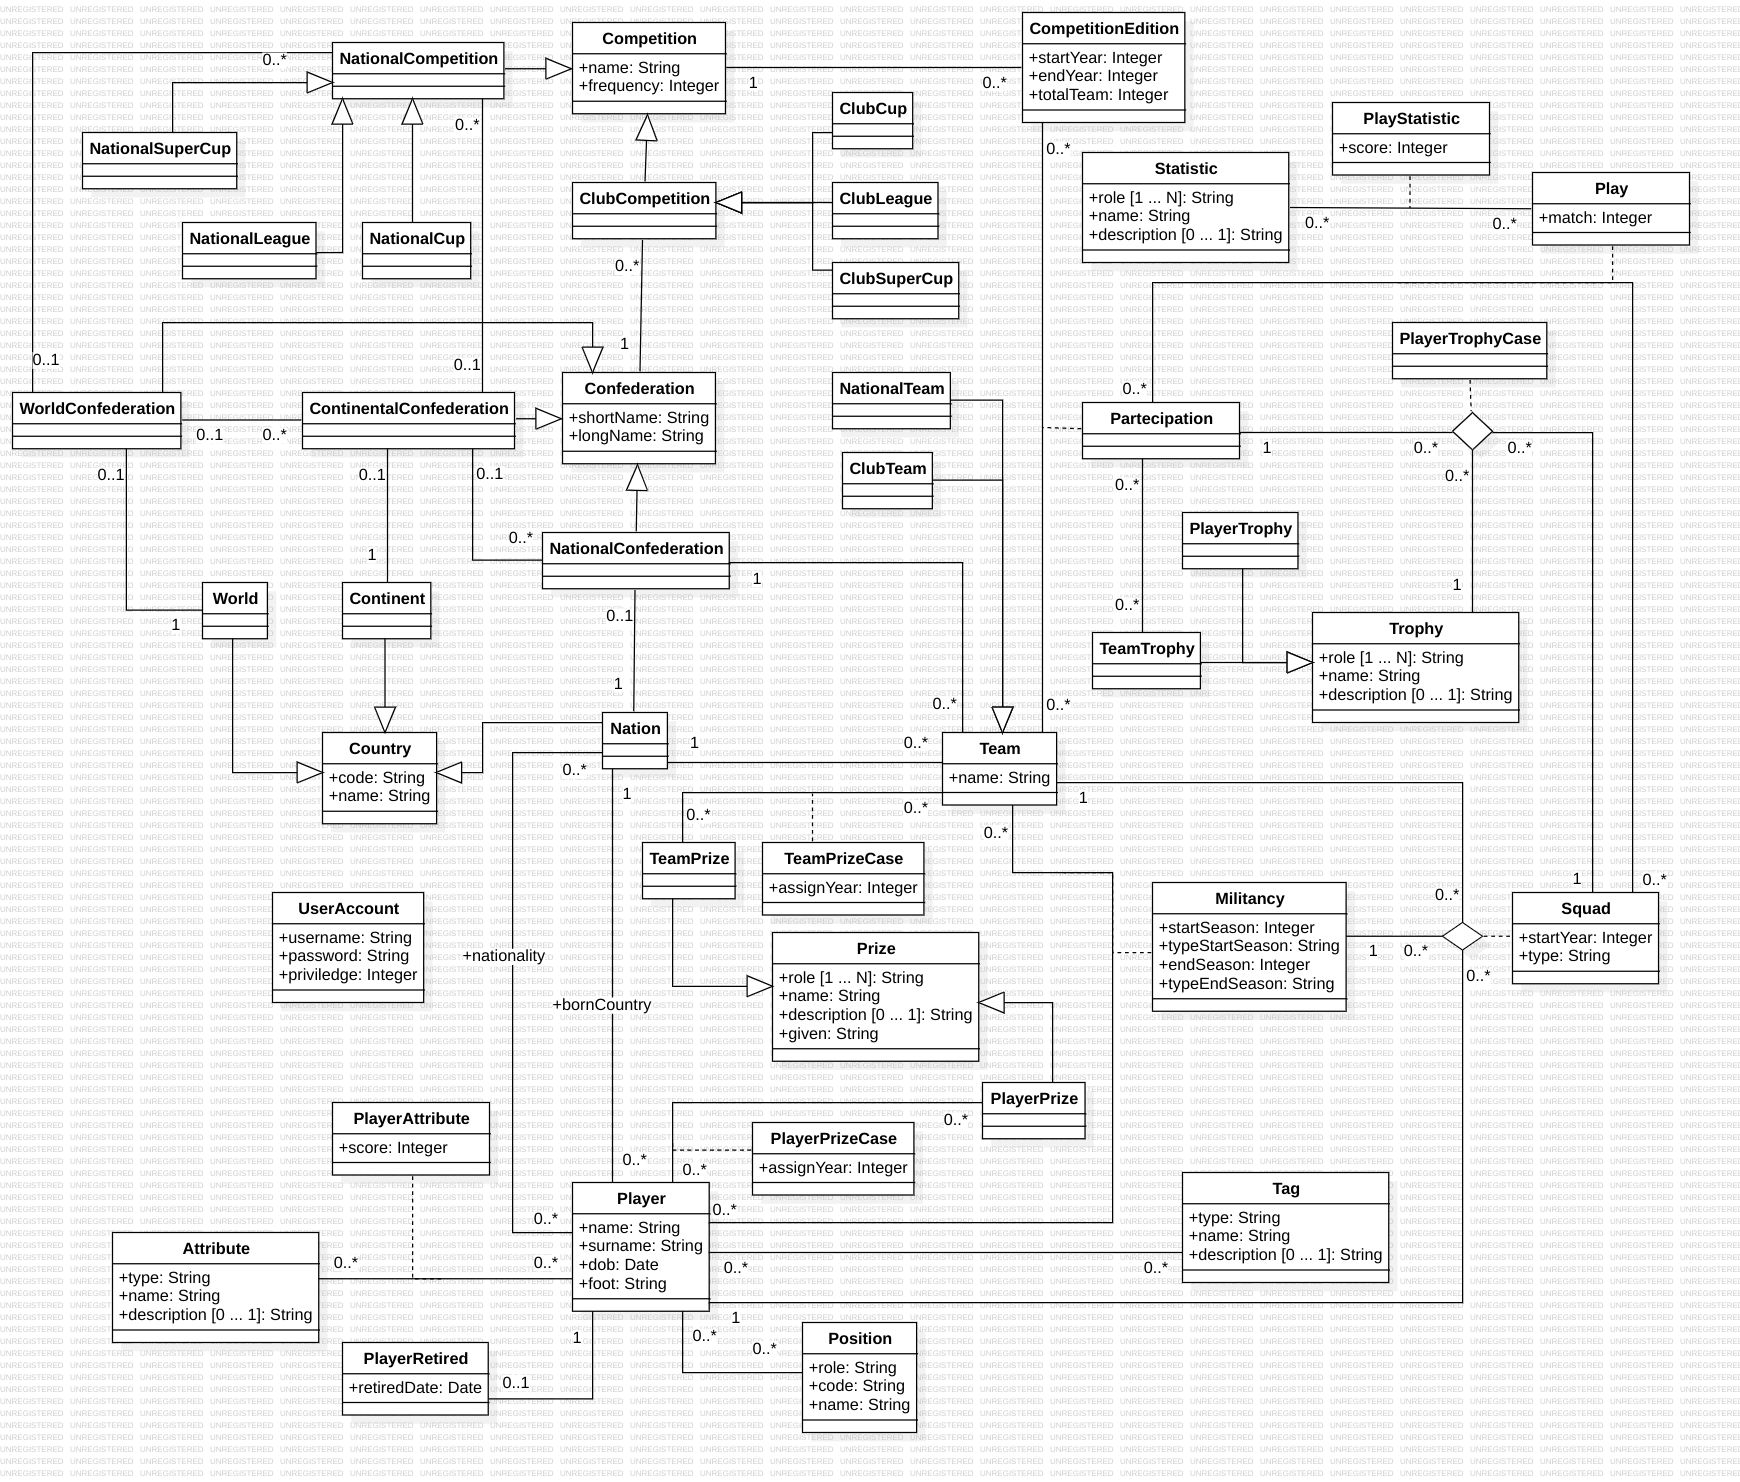
\includegraphics[width=\textwidth]{res/class_diagram_not_restr}
\newpage

\subsubsection{Analysis of the Class Diagram's restructuring}
\newpage
\subsubsection{Class Diagram ristrutturato}
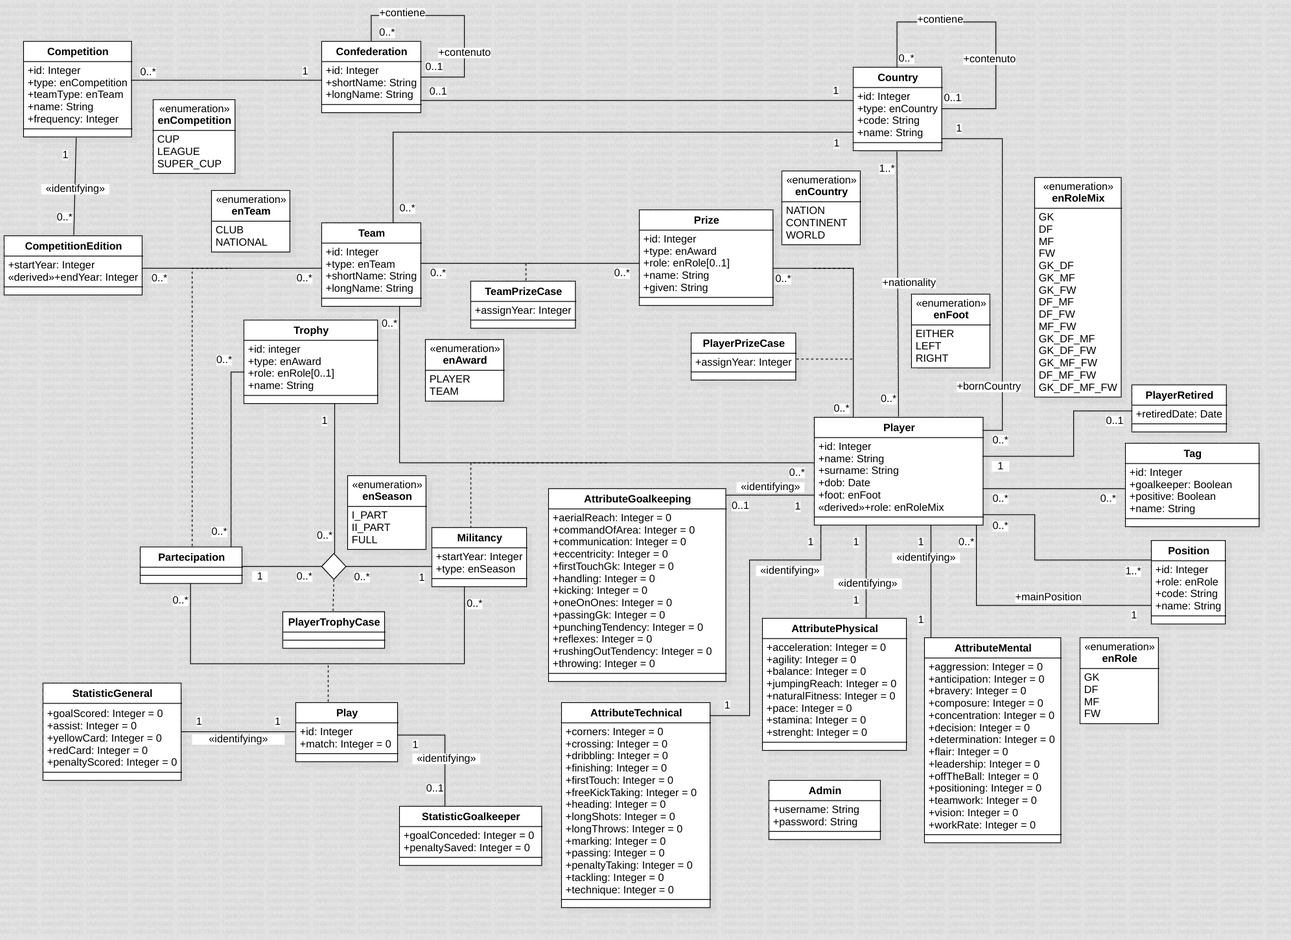
\includegraphics[scale= 0.242]{res/class_diagram_ristr}
\newpage

\subsubsection{Dizionario}

\begin{center}
	\textbf{Dizionario delle Classi}
\end{center}


\begin{tblr}{
    hlines = {0.9pt}, vlines = {0.9pt}, colspec = {X[l]X[l]X[l]}, column{1}= {100pt},
    width = \textwidth, cell{1}{1-3} = {blue!10!white}
}
	{
		Classe
	}
	&
	{
		Descrizione
	}
	&
	{
		Attributo
	}
	\\
	{
		Attribute
	}
	&
	{
		Rappresenta gli attributi di un calciatore.
	}
	&
	{
		\textbf{id}(Integer)[chiave surrogata]:\\Rappresenta
			l'identificativo di un Attributo.\\
		\medskip\textbf{type}(enFeature):\\Rappresenta
			il tipo di un Attributo.\\
		\medskip\textbf{name}(String)[chiave naturale]:
			\\Rappresenta il nome di un Attributo.\\
		\medskip\textbf{description}(String)[parziale]:
			\\Rappresenta la descrizione di un Attributo.
	}
	\\
	{
		Competition
	}
	&
	{
		Rappresenta le competizioni calcistiche.
	}
	&
	{
		\textbf{id}(Integer)[chiave surrogata]:\\Rappresenta
			l'identificativo di una Competizione.\\
		\medskip\textbf{type}(enCompetition):\\Rappresenta
			il tipo di una Competizione.\\
		\medskip\textbf{teamType}(enTeam):\\Rappresenta
			il tipo di squadra che può
			partecipare alla Competizione.\\
		\medskip\textbf{name}(String)[chiave naturale]:
			\\Rappresenta il nome di una Competizione.\\
		\medskip\textbf{frequency}(Integer):\\Rappresenta
			la frequenza di una Competizione.
	}
	\\
	{
		CompetitionEdition
	}
	&
	{
		Rappresenta le edizioni delle competizioni calcistiche.
	}
	&
	{
		\textbf{id}(Integer)[chiave surrogata]:\\Rappresenta
			l'identificativo di un'Edizione.\\
		\medskip\textbf{startYear}(Integer)[chiave parziale]:
			\\Rappresenta l'anno di inizio di un'Edizione.\\
		\medskip\textbf{endYear}(Integer)[chiave parziale]:
			\\Rappresenta l'anno di fine di un'Edizione.\\
		\medskip\textbf{totalTeam}(Integer):\\Rappresenta
			il numero di team che partecipano in un'Edizione.
	}
	\\
	{
		Confederation
	}
	&
	{
	Rappresenta le confederazioni calcistiche.
	}
	& 
	{
		\textbf{id}(Integer)[chiave surrogata]:\\Rappresenta
			l'identificativo di una Confederazione.\\
		\medskip\textbf{shortName}(String):\\Rappresenta
			il nome abbreviato di una Confederazione.\\
		\medskip\textbf{longName}(String)[chiave naturale]:
			\\Rappresenta il nome esteso di una Confederazione.
	}
	\\
\end{tblr}

\newpage

\begin{tblr}{
    hlines = {0.9pt}, vlines = {0.9pt}, colspec = {X[l]X[l]X[l]}, column{1}= {100pt},
    width = \textwidth
}
	{
		Country
	}
	&
	{
		Rappresenta i paesi in cui si gioca
		ufficialmente a calcio.
	}
	&
	{
		\textbf{id}(Integer)[chiave surrogata]:\\Rappresenta
			l'identificativo di un Paese.\\
		\textbf{type}(enCountry):\\Rappresenta
			il tipo di un Paese.\\
		\medskip\textbf{code}(String)[chiave naturale]:
			\\Rappresenta il codice ISO 3166-1 alpha-3
			di un Paese.\\
		\medskip\textbf{name}(String)[chiave naturale]:
			\\Rappresenta il nome di un Paese.
	}
	\\
	{
		Militancy
	}
	&
	{
		Rappresenta le militanze di un
		calciatore in una squadra.
	}
	&
	{
		\textbf{id}(Integer)[chiave surrogata]:\\Rappresenta
			l'identificativo di una Militanza.\\
		\medskip\textbf{dateRange}(daterange):\\Rappresenta
			il periodo di tempo in cui
			un calciatore era nella squadra.\\
		\medskip\textbf{match}:\\Rappresenta il numero
			di presenze di un Calciatore.
	}
	\\
	{
		MilitancyStatistic
	}
	&
	{
		Rappresenta l'associazione tra
		Militancy e Statistic.\\È una classe associativa.
	}
	& 
	{
		\textbf{score}(Integer)[derivato]:\\Rappresenta
			il valore di una Statistica per
			la Militanza associata.
	}
	\\
	{
		Partecipation
	}
	&
	{
		Rappresenta la partecipazione
		di un Team ad una CompetitionEdition.\\
		È una classe associativa.
	}
	&
	{
	
	}
	\\
	{
		Play
	}
	&
	{
		Rappresenta l'associazione tra
		Partecipation e PlayerPosition.\\
		È una classe associativa.
	}
	&
	{
		\textbf{id}(Integer)[chiave surrogata]:\\Rappresenta
			l'identificativo di un Gioco.\\
		\medskip\textbf{match}(Integer):\\Rappresenta
			il numero di presenze del Calciatore
			in quella Posizione,in una Squadra, per quella
			Edizione della competizione.
	}
	\\
	{
		PlayStatistic
	}
	&
	{	
		Rappresenta l'associazione tra Play e Statistic.\\
		È una classe associativa.
	}
	&
	{
		\textbf{score}(Integer):\\Rappresenta
			il valore di una Statistica per il Play associato.
	}
	\\
	{
		Player
	}
	&
	{
		Rappresenta i calciatori.
	}
	&
	{
		\textbf{id}(Integer)[chiave surrogata]:\\Rappresenta
			l'identificativo di un Calciatore.\\
		\medskip\textbf{name}(String):\\Rappresenta
			il nome di un Calciatore.\\
		\medskip\textbf{surname}(String):\\Rappresenta
			il cognome di un Calciatore.\\
		\medskip\textbf{dob}(Date):\\Rappresenta
			la data di nascita.\\
		\medskip\textbf{foot}(enFoot):\\Rappresenta
			il piede preferito di un Calciatore.\\
		\medskip\textbf{careerTime}(daterange):\\Rappresenta
			l'intervallo di tempo tra la data di debutto
			e la data di ritiro di un Calciatore.
	}
	\\
\end{tblr}

\newpage

\begin{tblr}{
    hlines = {0.9pt}, vlines = {0.9pt}, colspec = {X[l]X[l]X[l]}, column{1}= {100pt},
    width = \textwidth
}

	{
		PlayerAttribute
	}
	&
	{
		Rappresenta l'associazione tra Player e Attribute.\\
		È una classe associativa.
	}
	&
	{
		\textbf{score}(Integer):\\Rappresenta
			il valore di un Attributo associato al Calciatore.
	}
	\\
	{
		PlayerPosition
	}
	&
	{
		Rappresenta l'associazione tra Player e Position.\\
		È una classe associativa.
	}
	&
	{
		\textbf{match}(Integer)[derivato]:\\Rappresenta
			il numero di partite che un Calciatore gioca
			in una determinata Posizione.
	}
	\\
	{
		PlayerPrizeCase
	}
	&
	{
		Rappresenta la bacheca dei premi del calciatore.
	}
	&
	{
		\textbf{assignYear}(Integer):\\Rappresenta
			l'anno di assegnazione di un Premio.
	}
	\\
	{
		PlayerTrophyCase
	}
	&
	{
		Rappresenta la bacheca dei trofei di un calciatore.
	}
	&
	{
	
	}
	\\
	{
		Position
	}
	&
	{
		Rappresenta le posizioni di gioco di un Calciatore.
	}
	&
	{
		\textbf{id}(Integer)[chiave surrogata]:\\Rappresenta
			l'identificativo di una Posizione.\\
		\medskip\textbf{role}(enRole):\\Rappresenta
			il ruolo associato ad una Posizione.\\
		\medskip\textbf{code}(String)[chiave naturale]:
			\\Rappresenta il nome abbreviato di una Posizione.\\
		\medskip\textbf{name}(String)[chiave naturale]:
			\\Rappresenta il nome di una Posizione.
	}
	\\
	{
		Prize
	}
	&
	{
		Rappresenta i premi calcistici.
	}
	&
	{
		\textbf{id}(Integer)[chiave surrogata]:\\Rappresenta
			l'identificativo del Premio.\\
		\medskip\textbf{type}(enAward):\\Rappresenta
			il tipo del Premio.\\
		\medskip\textbf{role}(enRoleMix):\\Rappresenta
			i possibili ruoli che sono associati ad un Premio.\\
		\medskip\textbf{name}(String)[chiave naturale]:
			\\Rappresenta il nome del Premio.\\
		\medskip\textbf{description}(String)[parziale]:
			\\Rappresenta la descrizione del Premio.\\
		\medskip\textbf{given}(String):\\Rappresenta
			il nome della società calcistica
			che conferisce il Premio.
	}
	\\
	{
		Statistic
	}
	&
	{
		Rappresenta le statistiche di un calciatore.
	}
	&
	{
		\textbf{id}(Integer)[chiave surrogata]:\\Rappresenta
			l'identificativo della Statistica.\\
		\medskip\textbf{role}(enRoleMix):\\Rappresenta
			i ruoli associati alla Statistica.\\
		\medskip\textbf{name}(String):\\Rappresenta
			il nome della Statistica.\\
		\medskip\textbf{description}(String)[parziale]:
			\\Rappresenta la descrizione della Statistica.
	}
	\\
\end{tblr}

\newpage

\begin{tblr}{
    hlines = {0.9pt}, vlines = {0.9pt}, colspec = {X[l]X[l]X[l]}, column{1}= {100pt},
    width = \textwidth
}
	{
		Tag
	}
	&
	{
		Rappresenta i tag di un calciatore.
	}
	&
	{
		\textbf{id}(Integer)[chiave surrogata]:\\Rappresenta
			l'identificativo del Tag.\\
		\medskip\textbf{type}(enFeature):\\Rappresenta
			il tipo del Tag.\\
		\medskip\textbf{name}(String)[chiave naturale]:
			\\Rappresenta il nome del Tag.\\
		\medskip\textbf{description}(String)[parziale]:
			\\Rappresenta la descrizione del Tag.
	}
	\\
	{
		Team
	}
	&
	{
		Rappresenta le squadre di calcio.
	}
	&
	{
		\textbf{id}(Integer)[chiave surrogata]:\\Rappresenta
			l'identificativo della Squadra.\\
		\medskip\textbf{type}(enTeam):\\Rappresenta
			il tipo della Squadra.\\
		\medskip\textbf{name}(String)[chiave naturale]:
			\\Rappresenta il nome della Squadra.
	}
	\\
	{
		TeamPrizeCase
	}
	&
	{
		Rappresenta la bacheca dei premi della squadra.
	}
	&
	{
		\textbf{assignYear}(Integer):\\Rappresenta
			l'anno di assegnazione di un Premio.
	}
	\\
	{
		Trophy
	}
	&
	{
		Rappresenta i trofei calcistici.
	}
	&
	{
		\textbf{id}(Integer)[chiave surrogata]:\\Rappresenta
			l'identificativo del Trofeo.\\
		\medskip\textbf{type}(enAward):\\Rappresenta
			il tipo del Trofeo.\\
		\medskip\textbf{role}(enRoleMix):\\Rappresenta
			i possibili ruoli a cui è associato un Trofeo.\\
		\medskip\textbf{name}(String)[chiave naturale]:
			\\Rappresenta il nome del Trofeo.\\
		\medskip\textbf{description}(String)[parziale]:
			\\Rappresenta la descrizione del Trofeo.\\
	}
	\\
	{
		UserAccount
	}
	&
	{
		Rappresenta gli utenti dell'applicativo.
	}
	&
	{
		\textbf{username}(String)[chiave naturale]:\\Rappresenta
			l'username dell'Account dell'Utente.\\
		\medskip\textbf{password}(String):\\Rappresenta
			la password dell'Account dell'Utente.\\
		\medskip\textbf{priviledge}(Integer):\\Rappresenta
			i privilegi dell'Account dell'Utente.
	}
	\\
\end{tblr}

\newpage

\begin{center}
	\textbf{Dizionario delle Associazioni}
\end{center}


\begin{tblr}{
    hlines = {0.9pt}, vlines = {0.9pt}, colspec = {X[l]X[l]X[l]}, column{1}= {100pt},
    width = \textwidth, cell{1}{1-3} = {blue!10!white}
}

	{
		Nome
	}
	&
	{
		Descrizione
	}
	&
	{
		Classi in Relazione
	}
	\\
	{
		Nationality
	}
	&
	{
		Esprime le nazionalità di un calciatore.\\
		È una relazione N a N.
	}
	&
	{
		\textbf{Country [0 ... *]}:\\Indica che
			uno stesso paese può essere associato a più
			calciatore.\\
		\medskip\textbf{Player [0 ... *]}:\\Indica che
			un calciatore può avere più nazionalità.
	}
	\\
	{
		bornCountry	
	}
	&
	{
		Esprime il paese di nascita di un calciatore.\\
		È una relazione 1 a N.
	}
	&
	{
		\textbf{Country [0 ... *]}:\\Indica che
			un paese può essere il paese di nascita
			di più calciatori.\\
		\medskip\textbf{Player [1]}:\\Indica che
			un calciatore ha uno e un solo paese di nascita.
	}
	\\
	{
		Player-PlayerAttribute
	}
	&
	{
		Esprime il valore degli attributi di un calciatore.\\
		È una relazione 1 a N.
	}
	&
	{
		\textbf{Player [0 ... *]}:\\Indica che un Calciatore
			può aver zero o più valori di Attributi associati.\\
		\medskip\textbf{PlayerAttribute [1]}:\\Indica che 
			un valore di un Attributo deve essere associato
			ad uno e un solo Calciatore.
	}
	\\
	{
		PlayerAttribute-Attribute
	}
	&
	{
		Esprime a quale attributo si riferisce
		PlayerAttribute.\\È una relazione 1 a N.
	}
	&
	{
		\textbf{PlayerAttribute [1]}:\\Indica che un valore
			di PlayerAttribute è associato ad uno e un solo
			Attributo.\\
		\medskip\textbf{Attribute [0 ... *]}:\\Indica che un
			Attributo può avere più valori associati.
	}
	\\
	{
		Player-Tag
	}
	&
	{
		Esprime i Tag associati ad un Calciatore.\\
		È una relazione N a N.
	}
	&
	{
		\textbf{Player [0 ... *]}:\\Indica che un Calciatore
			può avere più Tag associati.\\
		\medskip\textbf{Tag [0 ... *]}\\Indica che
			uno stesso Tag può essere associato a
			più Calciatori.
	}
	\\
	{
		Player - PlayerTrophyCase
	}
	&
	{
		Esprime i trofei associati ad un calciatore.\\
		È una relazione 1 a N.
	}	
	&
	{
		\textbf{Player [0 ... *]}:\\Indica che un Calciatore
			può avere più Trofei associati.\\
		\medskip\textbf{PlayerTrophyCase [1]}:\\Indica che una
			bacheca si può riferire ad uno e un solo Calciatore.
	}
	\\
	{
		PlayerTrophyCase - Trophy
	}
	&
	{
		Esprime i trofei associati ad una bacheca.\\
		È una relazione 1 a N.
	}
	&
	{
		\textbf{PlayerTrophyCase [1]}:\\Indica che una bacheca
			si può riferire ad uno e un solo Trofeo.\\
		\medskip\textbf{Trophy [0 ... *]}:\\Indica che
			un Trofeo può avere più bacheche associate.
	}
	\\
\end{tblr}

\newpage

\begin{tblr}{
    hlines = {0.9pt}, vlines = {0.9pt}, colspec = {X[l]X[l]X[l]}, column{1}= {100pt},
    width = \textwidth
}

	{
		PlayerTrophyCase - Partecipation
	}
	&
	{
		Esprime le partecipazioni di una squadra
		ad una competizione edizione associate
		ad una bacheca.\\
		È una relazione 1 a N.
	}
	&
	{
		\textbf{PlayerTrophyCase [1]}:\\Indica che una bacheca
			si può riferire ad uno e un sola Partecipazione.
		\medskip\textbf{Partecipation [0 ... *]}:\\Indica che
			una Partecipazione può avere più bacheche associate.
	}
	\\
	{
		Player-PlayerPosition
	}
	&
	{
		Esprime il numero di partite che un Calciatore
		ha fatto in una certa posizione.\\
		È una relazione 1 a N.
		
	}
	&
	{
		\textbf{Player [0 ... *]}:\\Indica che un Calciatore
			può avere più posizioni di gioco associate.\\
		\medskip\textbf{PlayerPosition [1]}:\\Indica che
			il numero di partite di una posizione di gioco si
			può riferire ad uno e un solo Calciatore.
	}
	\\
	{
		PlayerPosition-Position
	}
	&
	{
		Esprime a quale posizione è associato
		il numero di partite di un Calciatore.\\
		È una relazione 1 a N.
	}
	&
	{
		\textbf{PlayerPosition [1]}:\\Indica che il numero
			di partite di una posizione di gioco si può riferire
			ad una e una sola posizione.\\
		\medskip\textbf{Position [0 ... *]}:\\Indica che
			una Posizione può avere più calciatori associati.
	}
	\\
	{
		Player-Militancy
	}
	&
	{
		Esprime le Militanze associate ad un Calciatore.\\
		È una relazione 1 a N.
	}
	&
	{
		\textbf{Player [0 ... *]}:\\Indica che il Calciatore
			può avere più Militanze associate.\\
		\medskip\textbf{Militancy [1]}:\\Indica che
			una Militanza si può riferire ad uno
			e un solo Calciatore.
	}
	\\
	{
		Militancy-Team
	}
	&
	{
		Esprime a quale Squadra una Militanza è associata.\\
		È una relazione 1 a N.
	}
	&
	{
		\textbf{Militancy [1]}:\\Indica che una Militanza
			si può riferire ad una e una sola Squadra.\\
		\medskip\textbf{Team [0 ... *}:\\Indica che una Squadra
			può avere più Militanze associate.
	}
	\\
	{
		Player-PlayerPrizeCase
	}
	&
	{
		Esprime i premi associati ad un Calciatore
		nella Bacheca.\\È una relazione 1 a N.
	}
	&
	{
		\textbf{Player [0 ... *]}:\\Indica che un Calciatore
			può avere più premi associati in una Bacheca.
		\medskip\textbf{PlayerPrizeCase [1]}:\\Indica che una
			Bacheca si può riferire ad un e un solo Calciatore.
	}
	\\
	{
		PlayerPrizeCase-Prize
	}
	&
	{
		Esprime i Premi ai quali è associata una Bacheca.\\
		È una relazione 1 a N.
	}
	&
	{
		\textbf{PlayerPrizeCase [1]}:\\Indica che una Bacheca
			si può riferire ad un e un solo Premio.\\
		\medskip\textbf{Prize [0 ... *]}:\\Indica che un Premio
			può avere più Bacheche associate.
	}
	\\
	{
		Team-Country
	}
	&
	{
		Esprime la nazionalità di una Squadra.\\
		È una relazione 1 a N.
	}
	&
	{
		\textbf{Team [1]}:\\Indica che una Squadra si riferisce
			ad un e un solo paese.\\
		\medskip\textbf{Country [0 ... *]}:\\Indica che un Paese
			può avere più Squadre associate.
	}
	\\
\end{tblr}

\newpage

\begin{tblr}{
    hlines = {0.9pt}, vlines = {0.9pt}, colspec = {X[l]X[l]X[l]}, column{1}= {100pt},
    width = \textwidth
}

	{
		Team-Confederation
	}
	&
	{
		Esprime la Confederazione di cui una Squadra è membra.\\
		È una relazione 1 a N.
	}
	&
	{
		\textbf{Team [1]}:\\Indica che una Squadra si riferisce
			ad una e una sola Confederazione.\\
		\medskip\textbf{Confederation [0 ... *]}:\\Indica che
			una Confederazione può avere più Squadre associate.
	}
	\\
	{
		Team-Partecipation	
	}
	&
	{
		Esprime le edizioni delle Competizioni a cui una Squadra
		Partecipa.\\È una relazione 1 a N.
	}
	&
	{
		\textbf{Team [0 ... *]}:\\Indica che una Squadra può
			partecipare a più Competizioni Edizioni.\\
		\medskip\textbf{Partecipation [1]}:\\Indica che una
			Partecipazione può riferirsi ad una e una sola
			Squadra.
	}
	\\
	{
		Partecipation-CompetitionEdition
	}
	&
	{
		Esprime a quali Edizioni di una Competizione una
		Partecipazione di una Squadra si riferisce.\\
		È una relazione 1 a N.
	}
	&
	{
		\textbf{Partecipation [1]}:\\Indica che
			una Partecipazione può riferirsi ad una e una sola
			Edizione di una Competizione.\\
		\medskip\textbf{CompetitionEdition [0 ... *]}:\\Indica
			che una Edizione di una Competizione può avere più
			Partecipazioni associate.
	}
	\\
	{
		Team-TeamPrizeCase
	}
	&
	{
		Esprime i premi associati ad una Squadra
		in una Bacheca.\\È una relazione 1 a N.
	}
	&
	{
		\textbf{Team [0 ... *]}:\\Indica che una Squadra
			può avere più premi associati in una Bacheca.\\
		\medskip\textbf{TeamPrizeCase [1]}:\\Indica che una
			Bacheca si può riferire ad una e una sola Squadra.
	}
	\\
	{
		TeamPrizeCase-Prize	
	}
	&
	{
		Esprime i Premi ai quali è associata una Bacheca.\\
		È una relazione 1 a N.
	}
	&
	{
		\textbf{TeamPrizeCase [1]}:\\Indica che una Bacheca
			si può riferire ad un e un solo Premio.\\
		\medskip\textbf{Prize [0 ... *]}:\\Indica che un Premio
			può avere più Bacheche associate.
	}
	\\
	{
		Confederation-Country
	}
	&
	{
		Esprime l'appartenza di una Confederazione
		ad un unico Paese e viceversa.\\È una relazione 1 a 1.
	}
	&
	{
		\textbf{Confederation [1]}:\\Indica che
			una Confederazione si può riferire
			ad un e un solo Paese.\\
		\medskip\textbf{Country [1]}:\\Indica che un Paese
			si può riferire ad una e una sola Confederazione.
	}
	\\
	{
		Membro
	}
	&
	{
		Esprime la possibilità di una confederazione di
		avere come membri altre confederazioni, o essere
		membro a sua volta.\\
		È una relazione 1 a N.
	}
	&
	{
		\textbf{Confederation [0 ... 1]} ruolo (contenuto):\\
			Indica che una Confederazione può o non può essere
			membra di un'altra Confederazione.
		\medskip\textbf{Confederation [0 ... *]}
			ruolo (contiene):\\
			Indica che una Confederazione può avere più
			Confederazioni come membri.
	}
	\\
	{
		Confederation-Competition
	}
	&
	{
		Esprime la capacità di una Confederazione di creare
		Competizioni.\\È una relazione 1 a N.
	}
	&
	{
		\textbf{Confederation [0 ... *]}:\\Indica che una
			Confederazione può creare più Competizioni.
		\medskip\textbf{Competition [1]}:\\Indica che una
			Competizione si riferisce ad una e una sola
			Confederazione.
	}
	\\
\end{tblr}

\newpage

\begin{tblr}{
    hlines = {0.9pt}, vlines = {0.9pt}, colspec = {X[l]X[l]X[l]}, column{1}= {100pt},
    width = \textwidth
}
	{
		Competition-CompetitionEdition
	}
	&
	{
		Esprime la capacità di una Competizione di avere
		Edizioni.\\È una relazione 1 a N.
		
	}
	&
	{
		\textbf{Competition [0 ... *]}:\\Indica che una
			Competizione può avere più Edizioni associate.\\
		\medskip\textbf{CompetitionEdition [1]}:\\Indica che
			una Edizione si riferisce ad una e una sola
			Competizione
	}
	\\
	{
		Trophy-Partecipation
	}
	&
	{
		Esprime la bacheca dei trofei di una Squadra.\\
		È una relazione N a N.
	}
	&
	{
		\textbf{Trophy [0 ... *]}:\\Indica che un Trofeo
			può avere più Partecipazioni di una Squadra ad
			una Edizione associati.\\
		\medskip\textbf{Partecipation [0 ... *]}:\\Indica che
			una Partecipazione può avere più trofei associati.
	}
	\\
	{
		Play-PlayerPosition
	}
	&
	{
		Esprime un calciatore in che posizione ha giocato.	\\
		È una relazione 1 a N.
	}
	&
	{
		\textbf{Play [1]}:\\Indica che un Gioco si riferisce
			a una e una sola Posizione di gioco del Calciatore.
		\medskip\textbf{PlayerPosition [0 ... *]}:\\Indica che
			uno stesso Calciatore con la stessa
			Posizione di gioco può giocare più volte.
	}
	\\
	{
		Play-Partecipation
	}
	&
	{
		Esprime una squadra in che competizione ha giocato.\\
		È una relazione 1 a N.
	}
	&
	{
		\textbf{Play [1]}:\\Indica che un Gioco si riferisce
			a una e una sola Partecipazione.\\
		\medskip{Partecipation [0 ... *]}:\\Indica che una
			Partecipazione può avere più Giochi associati.
	}
	\\
	{
		Play-PlayStatistic
	}
	&
	{
		Esprime la capacità di un Gioco di poter avere
		valori di Statistiche associati.\\
		È una relazione 1 a N.
	}
	&
	{
		\textbf{Play [0 ... *]}:\\Indica che un Gioco può
			avere più valori di Statistiche associati.\\
		\medskip\textbf{PlayStatistic [1]}:\\Indica che
			il valore di una Statistica si riferisce ad
			uno e un solo Gioco.
	}
	\\
	{
		PlayStatistic-Statistic
	}
	&
	{
		Esprime la capacità delle Statistiche di poter avere
		più valori per il Gioco associati.\\
		È una relazione 1 a N.
	}
	&
	{
		\textbf{PlayStatistic [1]}:\\Indica che un valore
			di una Statistica si riferisce ad una e una sola
			Statistica.\\
		\medskip\textbf{Statistic [0 ... *]}:\\Indica che
			una Statistica può avere più valori associati.
	}
	\\
	{
		Statistic-MilitancyStatistic
	}
	&
	{
		Esprime la capacità delle Statistiche di poter avere
		più valori per la Militanza associati.\\
		È una relazione 1 a N.
	}
	&
	{
		\textbf{Statistic [0 ... *]}:\\Indica che una Statistica
			può avere più valori associati.\\
		\medskip\textbf{MilitancyStatistic [1]}:\\Indica che
			un valore di una Statistica si riferisce
			ad una e una sola Statistica.
			
	}
	\\
	{
		MilitancyStatistic-Militancy
	}
	&
	{
		Esprime la capacità di una Militanza di poter avere
		più valori di Statistiche associati.\\
		È una relazione 1 a N.
	}
	&
	{
		\textbf{MilitancyStatistic [1]}:\\Indica che
			un valore di una Statistica si riferisce
			ad una e una sola Militanza.\\
		\medskip\textbf{Militancy [0 ... *]}:\\Indica che
			una Militanza può avere più valori associati.
	}
	\\
\end{tblr}
%\newpage
\section{Object Orientation}
\newpage
\subsection{Analisi dei Requisiti}

Nell'affrontare questo progetto abbiamo Nell'affrontare questo progetto abbiamo deciso - seguendo i suggerimenti dei Docenti -, di svolgere
la traccia proposta entro una cornice più ampia, preservando il ruolo centrale delle entità-calciatori,
ma ponendole al centro di un contesto più complesso, rappresentativo dell'intero mondo calcistico.

A questo scopo, abbiamo effettuato una serie di indagini e ricerche sui principali siti di informazione riguardanti il calcio. Segnatamente, ci siamo basati sulle informazioni reperibili da Wikipedia, siti ufficiali delle principali confederazioni calcistiche, Transfermarkt, Fantagazzetta, FootballManager e vari altri siti e giornali di argomento calcistico.

Con non poca difficoltà abbiamo cercato di astrarre quelle che, a una prima analisi, abbiamo giudicato essere le
caratteristiche fondamentali del sistema-calcio nel mondo reale e di configurarle, al meglio delle nostre
possibilità, nel progetto assegnatoci.

\bigskip
\bigskip

Un primo aspetto concettuale - che sin da subito è risultato evidente - è che il sistema-calcio è
gerarchico, strutturato come un vero e proprio governo e costituito da confederazioni internazionali,
federazioni nazionali e leghe calcistiche (es. FIFA, UEFA, COMBEBOL, FIGC, \dots), che definiscono
le regole del gioco, organizzano le varie competizioni e sono pertanto il fulcro dell'intero sistema.

Per semplicità, a partire da questo momento con il termine "confederazione" faremo
riferimento indistintamente a confederazioni, federazioni, leghe e a qualsiasi altro ente
organizzativo che svolga un ruolo attivo nella gestione della struttura del sistema-calcio.

Ogni confederazione calcistica è associata con uno ed un solo paese.
\newline
Come per le confederazioni, trasporremo su di un livello di astrazione superiore anche il concetto di paese.
Identificheremo come "paese" i concetti di regione, nazione, continente e persino il mondo intero.

Data la relazione che intercorre tra un paese ed una confederazione calcistica, queste ultime
potranno essere suddivise in tre grandi categorie:

\begin{itemize}
	\item Confederazioni nazionali;
	\item Confederazioni continentali;
	\item Confederazioni mondiali.
\end{itemize}

Sottolineiamo che tale suddivisione opera una certa semplificazione, in quanto
esistono confederazioni subcontinentali, confederazioni regionali e così via; ci è sembrato
superfluo elevare ulteriormente la granularità della nostra analisi.

Un'ulteriore aspetto concettuale che abbiamo rilevato in corso di ricerca è che -
come già accennato - le confederazioni sono organizzate in ordine gerarchico: le confederazioni
nazionali fanno parte di confederazioni continentali, che a loro volta sono
membri di confederazioni mondiali (es. la FIGC è membro della UEFA che a sua volta è membro
della FIFA).
Questo pattern si ripresenta per la quasi totalità delle confederazioni che abbiamo osservato:
le uniche e rare eccezioni fanno capo a confederazioni minori isolate, esterne alla FIFA,
che quindi non sono in associazione con nessun'altra confederazione.
Dalle ricerche effettuate abbiamo notato che a tutti gli effetti il sistema-calcio fa capo
alla FIFA e pertanto si è deciso di escludere il calcio esterno alla FIFA.


È indiscutibile che il concetto di confederazione calcistica, insieme a quello di paese,
formino la base sulla quale poggia tutta l'organizzazione calcistica mondiale.

\bigskip
\bigskip

Come detto in precedenza, ciascuna confederazione organizza diverse competizioni calcistiche.
Una competizione calcistica può essere analizzata secondo diversi criteri;
se consideriamo come elemento discriminante il tipo di squadra che può parteciparvi, è possibile
dividere le competizioni calcistiche in due categorie:
\begin{itemize}
	\item Competizioni per squadre di tipo club;
	\item Competizioni per squadre di tipo nazionale.
\end{itemize}

Tuttavia, se l'elemento discriminante è il format che caratterizza una competizione
calcistica, queste possono essere raggruppate in tre categorie:
\begin{itemize}
	\item Competizioni di tipo campionato;
	\item Competizioni di tipo torneo;
	\item Competizioni di tipo supercoppa.
\end{itemize}

In effetti, l'analisi delle competizioni calcistiche è ben più complessa di quella che stiamo descrivendo. Infatti, una competizione può svolgersi anche secondo una formula (girone all'italiana, eliminazione diretta, \dots),
che può variare in base all'edizione della competizione che si sta considerando,
e secondo cui può variare anche il numero di partecipanti. Risulta pertanto estremamente complicato astrarre coerentemente questo insieme di informazioni.

Nonostante le difficoltà, abbiamo cercato di conciliare e preservare entrambi i punti di vista sulle
competizioni calcistiche e, seguendo la traccia, abbiamo selezionato come preminente uno
dei due.

Nella traccia si fa un chiaro riferimento alle squadre di calcio, e pertanto ci è sembrato
più corretto prediligere la prospettiva che mettesse maggiormente in risalto questo aspetto;
pertanto, dati i nostri scopi, il concetto di competizione calcistica sarà in primo luogo
considerato in base al tipo di squadra che può parteciparvi, e solo in secondo luogo
in base al tipo di format.

Vale la pena fare un'importante precisazione: una confederazione nazionale non potrà organizzare competizioni
calcistiche per squadre di tipo nazionale.

\bigskip
\bigskip

Come ben noto, ogni competizione ha diverse edizioni, ciascuna delle quali si svolge entro
una specifica stagione calcistica.

Dalle ricerche effettuate è emerso che, nell'ambito di un'unica confederazione organizzativa e di uno specifico format, è possibile classificare le edizioni competitive per gradi di importanza (es. nella FIGC la serie A è il campionato di "primo
livello", la serie B il campionato di "secondo livello").

Abbiamo concluso che non può esistere una squadra di calcio che, nella
stessa stagione, partecipi a due diverse competizioni dello stesso format orgnizzate dalla stessa
confederazione.

Una stagione calcistica è a tutti gli effetti l'unità di misura temporale del calcio. E' scandita in un periodo che intercorre tra due anni consecutivi (es. Stagione 2023-2024).
Per le competizioni di squadre di tipo nazionale, il concetto di stagione calcistica
coincide con la durata di un anno solare (es. Stagione 2023-2023).

In una qualsiasi istanza di un'edizione competitiva, al termine delle competizioni previste, ad alcune squadre tra le partecipanti vengono assegnati dei trofei, in base alla loro posizione in classifica.

Un trofeo, quindi, risulta concettualmente associato a una specifica edizione di una competizione
calcistica; d'altra parte, le nostre ricerche hanno evidenziato la presenza di trofei calcistici
indipendenti dalle competizioni.


Pertanto, dal punto di vista astratto, si è reso necessario operare una distinzione tra i trofei calcistici
che saranno sempre correlati a delle competizioni, e premi calcistici che, invece
occorrono in maniera indipendente.

Un ultimo concetto chiave relativo al mondo del calcio è quello di "squadra di calcio".
Una squadra di calcio appartiene a una nazione e fa sempre parte della
confederazione della nazione a cui è associata.
Una squadra può far parte di due grandi categorie:
\begin{itemize}
	\item Squadra di calcio di tipo club;
	\item Squadra di calcio di tipo nazionale.
\end{itemize}

Dalle nostre ricerche è inoltre risultato che una squadra di calcio può partecipare
solo alle competizioni (del tipo di squadra corrispondente) organizzate dalla confederazione
di cui è membro o da confederazioni che contengono la confederazione calcistica di cui
è membro (es. la Salernitana, squadra di calcio di tipo club che appartiene alla FIGC,
può partecipare alle competizioni organizzate dalla FIGC, ma anche a quelle organizzate
dalla UEFA (Professore, la Salernitana in Europa è e rimarrà un sogno!),
ma non alle competizioni organizzate dalla COMBEBOL).

Un'ultima precisazione: abbiamo deciso di escludere dalla nostra trattazione sia il calcio
femminile che il calcio giovanile, non rappresentando questi un ampliamento efficace del presente progetto.
Aggiungeremo che, in ogni caso, sarebbe stato gestibile in modo essenzialmente identico, con la sola aggiunta di qualche attributo; è stato pertanto ritenuto uno sforzo inutile.

\bigskip
\bigskip

Questo è, in estrema sintesi, l'arricchimento che abbiamo deciso di conferire al nostro progetto.
Ricordiamo però che il principale scopo del nostro lavoro è costruire un sistema informativo
per la gestione di calciatori di tutto il mondo.

Le ricerche effettuate e le conclusioni a cui siamo giunti non rappresentano
un mero esercizio di stile, ma ci permetteranno di disporre di una descrizione più sofisticata dei singoli calciatori - a scapito della semplicità formale del progetto.

\bigskip
\bigskip

Ogni calciatore avrà una nazione di nascita, una o più nazionalità e,
come indicato da traccia, una carriera durante la quale può militare in diverse
squadre di calcio.

A questo proposito è doveroso fare una importante precisazione. Vista la natura più dettagliata
della nostra visione del progetto, anche il concetto di militanza di un calciatore in una squadra
di calcio sarà più dettagliato.

Il nostro concetto astratto di militanza sarà la presenza di un calciatore in una squadra
durante una stagione calcistica, visto che, come detto, la stagione è l'unità di misura
temporale del mondo calcio.

Abbiamo deciso quindi di non considerare la data di inizio e fine di una certa militanza in
quanto al nostro livello di dettaglio è impossibile da gestire in modo coerente e corretto,
mantenendo anche un certo livello di astrazione.
Infatti, a seguito delle nostre ricerche abbiamo notato che il regolamento vigente
prevede che un cambio di militanza di un calciatore da una squadra ad un'altra
possa avvenire solo in particolari periodi di tempo, detti "finestre di mercato",
che per altro sono variabili in base alla stagione considerata e alla confederazione
calcistica cui fanno riferimento; ecco il motivo per il quale non è possibile utilizzare
le date come richiesto da traccia.
Sarebbe, infatti, impossibile controllare correttamente le variazioni della militanza di un calciatore
durante la sua carriera e potrebbe accadere che il calciatore in questione in una stagione
possa militare in più squadre di quelle possibili secondo il regolamento.

Ultimo appunto riferito alla militanza: per le militanze di calciatori in squadre di tipo
nazionale abbiamo seguito le indicazioni del regolamento corrente, secondo il quale un calciatore
può giocare solo per una squadra nazionale in tutta la sua carriera. Tale squadra
deve rappresentare una nazione di cui il calciatore sia cittadino.

Abbiamo quindi gestito le militanze per stagione calcistica.

Durante una militanza in una squadra, un calciatore potrà giocare un certo numero di
partite di un'edizione di una competizione cui partecipa la squadra in cui milita.

Al gioco di un calciatore in un'edizione di una competizione calcistica saranno associate
alcune statistiche.

Dal punto di vista astratto, una statistica di gioco è un qualsiasi evento misurabile durante
una partita - e statisticamente rilevante - relativo al gioco del calcio
(numero di goal, numero di assist, \dots).

Visto lo scopo del nostro progetto, si è stabilito di uniformare le statistiche, definendo una
lista di statistiche predefinite generali ed altre specifiche per i calciatori che giocano
come portieri.

Similmente a quello che accade per una squadra, anche un calciatore potrà vincere dei trofei.
Come da traccia, tali trofei potranno essere individuali o di squadra.
Pertanto un trofeo potrà appartenere a due categorie:
\begin{itemize}
	\item Trofeo individuale;
	\item Trofeo di squadra.
\end{itemize}

Più specificamente, i trofei di squadra saranno vinti da una squadra e, per transitività, poi
assegnati a tutti i calciatori che militano nella suddetta squadra durante quella stagione.
Quelli individuali, invece, potranno essere vinti solo dai singoli calciatori.

Analogamente un calciatore potrà vincere premi calcistici individuali (es. Pallone d'oro).
Anche in questo caso, i premi potranno appartenere a due categorie:
\begin{itemize}
	\item Premio individuale;
	\item Premio di squadra.
\end{itemize}

Con l'importante differenza che un premio di squadra non potrà essere assegnato ad un
calciatore.

Un calciatore è inoltre caratterizzato da una posizione di gioco principale e possibilmente da una
serie di posizioni di gioco alternative che ne andranno a definire i ruoli.

Inoltre, come da traccia, ad un calciatore possono essere associati dei tag che mettono in
risalto le specialità del calciatore.

In aggiunta a ciò, prendendo ispirazione da FootballManager, si è deciso di includere nella
descrizione del calciatore anche una serie di attributi che ne descrivano in modo quantitativo
le capacità sotto diversi aspetti.

Infine, un calciatore potrà ritirarsi dal gioco in una certa data.

\bigskip
\bigskip

Come da traccia, tale DataBase sarà accessibile mediante un applicativo da diversi utenti.
In base al tipo di utente, e conseguentemente al suo livello di privilegio, saranno possibili
determinate azioni sul database.

Un utente semplice potrà solo visualizzare dati ed informazioni contenuti nel DataBase.
Un utente di tipo amministratore potrà anche modificare i dati e le informazioni relative a
squadre di calcio e calciatori (come richiesto da traccia).

Pertanto è stato scelto di rendere alcune informazioni permanenti, in modo tale da assicurare
che la struttura portante del DataBase, che rappresenta il sistema calcio, rimanga invariata.

È chiaro che poi il responsabile del DataBase potrà invece effettuare tutte le modifiche del caso.
\subsection{Progettazione Concettuale}

\newpage

\subsubsection{Class Diagram non ristrutturato}

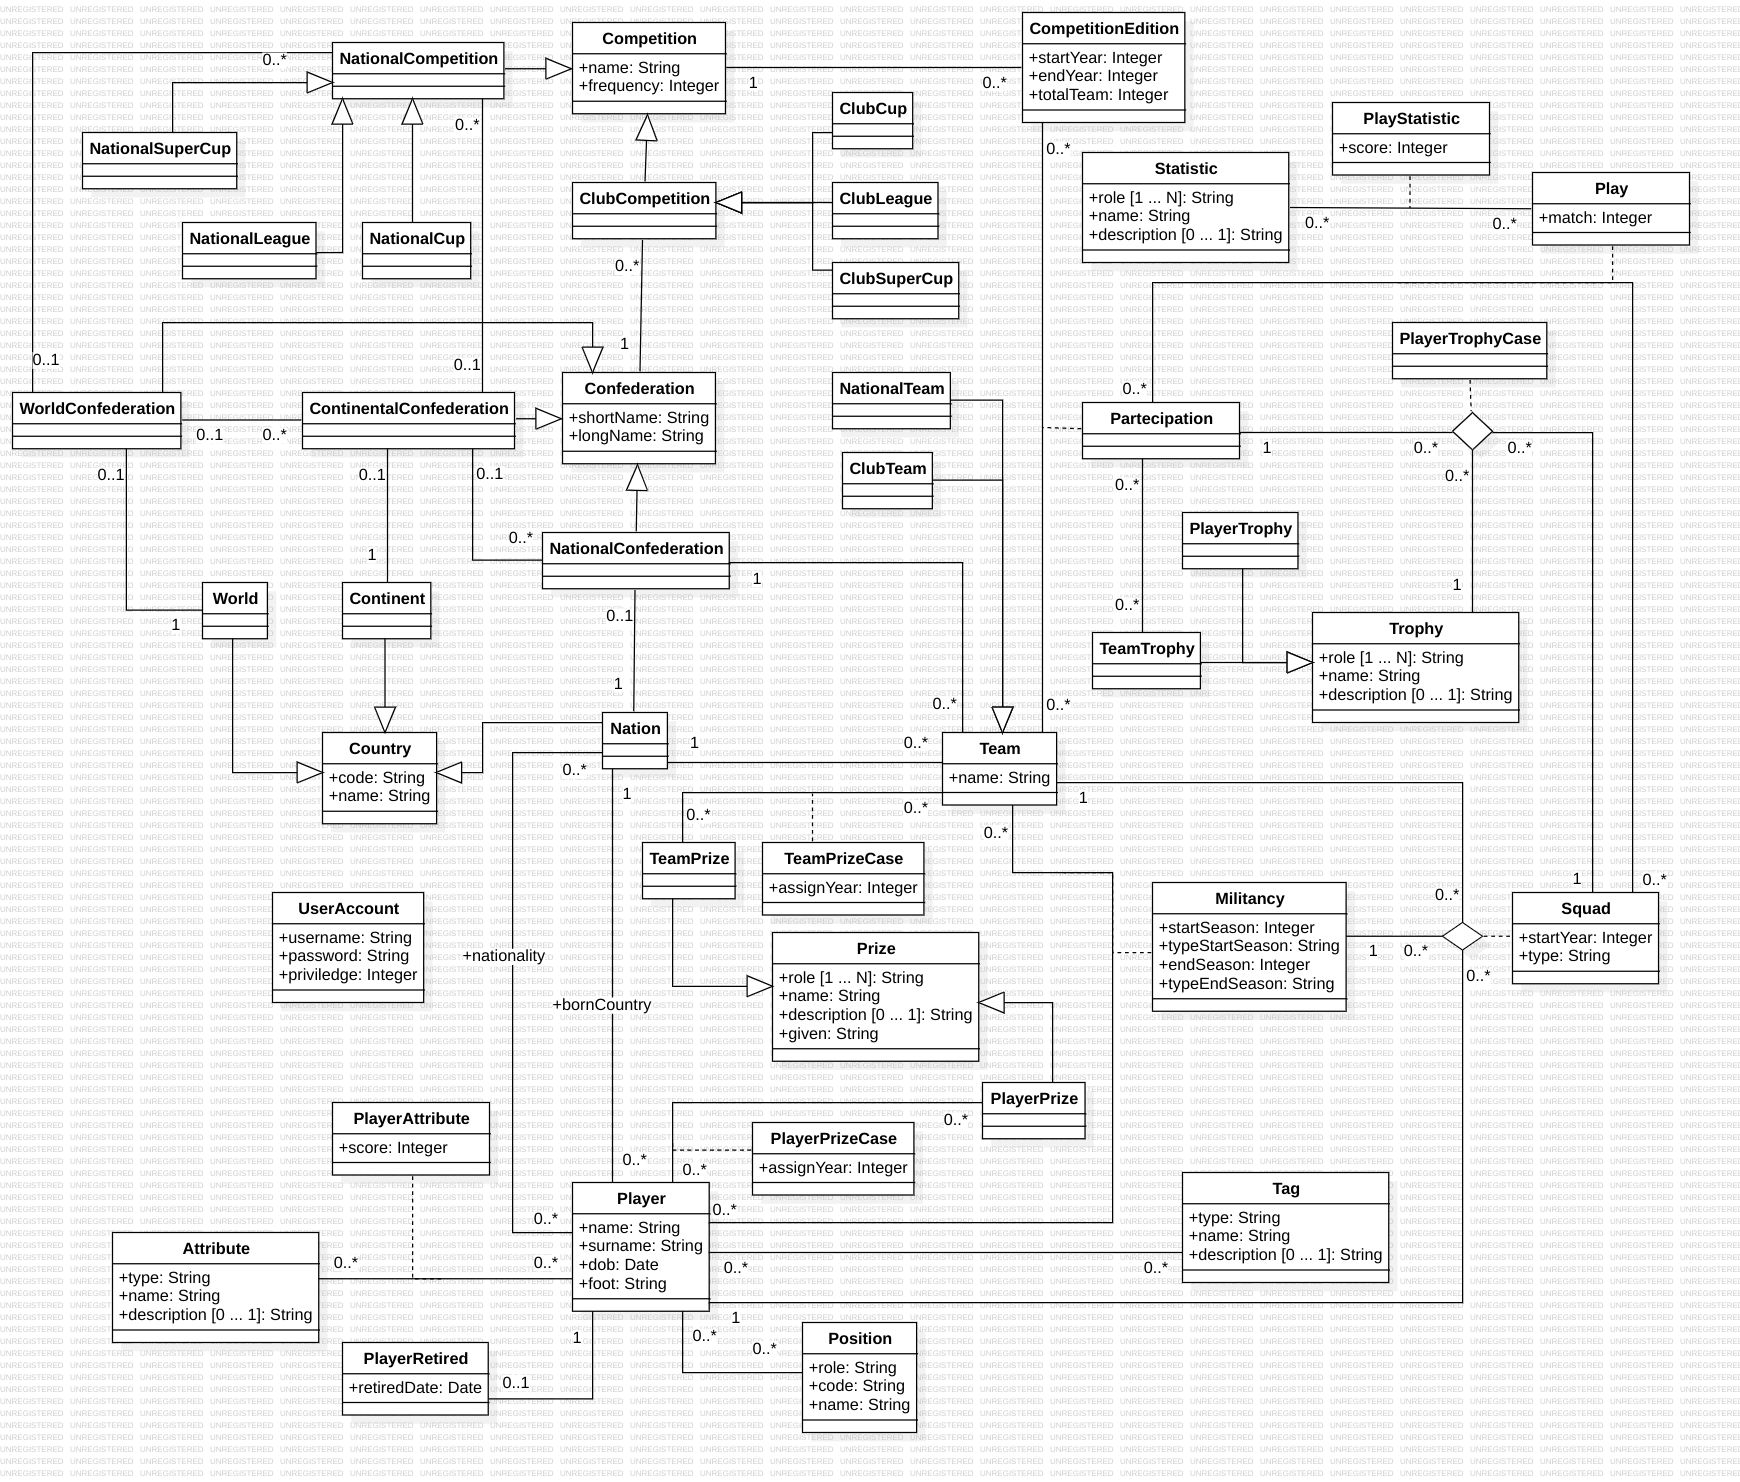
\includegraphics[width=\textwidth]{res/class_diagram_not_restr}
\newpage

\subsubsection{Analysis of the Class Diagram's restructuring}
\newpage
\subsubsection{Class Diagram ristrutturato}
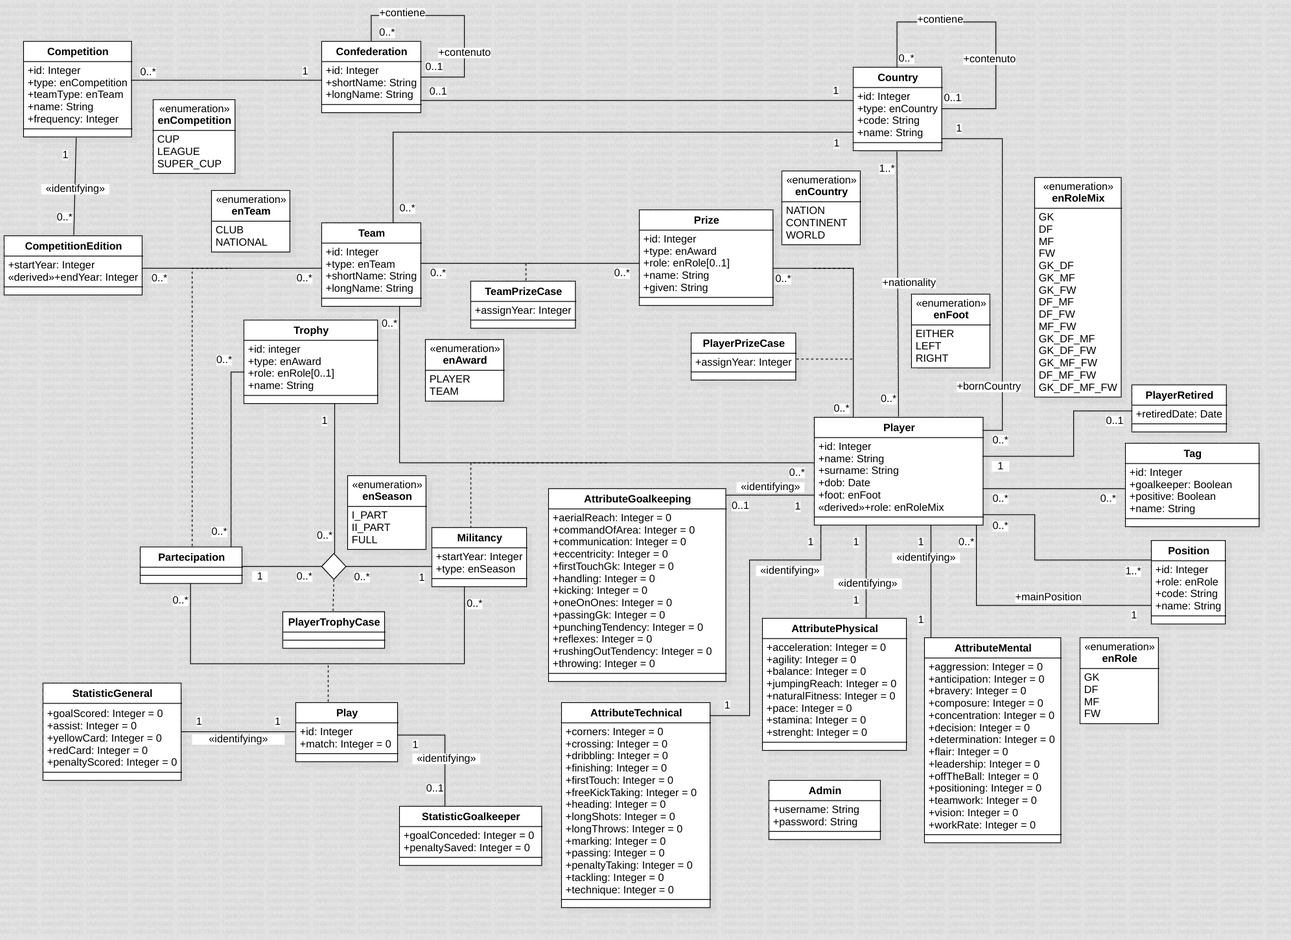
\includegraphics[scale= 0.242]{res/class_diagram_ristr}
\newpage

\subsubsection{Dizionario}

\begin{center}
	\textbf{Dizionario delle Classi}
\end{center}


\begin{tblr}{
    hlines = {0.9pt}, vlines = {0.9pt}, colspec = {X[l]X[l]X[l]}, column{1}= {100pt},
    width = \textwidth, cell{1}{1-3} = {blue!10!white}
}
	{
		Classe
	}
	&
	{
		Descrizione
	}
	&
	{
		Attributo
	}
	\\
	{
		Attribute
	}
	&
	{
		Rappresenta gli attributi di un calciatore.
	}
	&
	{
		\textbf{id}(Integer)[chiave surrogata]:\\Rappresenta
			l'identificativo di un Attributo.\\
		\medskip\textbf{type}(enFeature):\\Rappresenta
			il tipo di un Attributo.\\
		\medskip\textbf{name}(String)[chiave naturale]:
			\\Rappresenta il nome di un Attributo.\\
		\medskip\textbf{description}(String)[parziale]:
			\\Rappresenta la descrizione di un Attributo.
	}
	\\
	{
		Competition
	}
	&
	{
		Rappresenta le competizioni calcistiche.
	}
	&
	{
		\textbf{id}(Integer)[chiave surrogata]:\\Rappresenta
			l'identificativo di una Competizione.\\
		\medskip\textbf{type}(enCompetition):\\Rappresenta
			il tipo di una Competizione.\\
		\medskip\textbf{teamType}(enTeam):\\Rappresenta
			il tipo di squadra che può
			partecipare alla Competizione.\\
		\medskip\textbf{name}(String)[chiave naturale]:
			\\Rappresenta il nome di una Competizione.\\
		\medskip\textbf{frequency}(Integer):\\Rappresenta
			la frequenza di una Competizione.
	}
	\\
	{
		CompetitionEdition
	}
	&
	{
		Rappresenta le edizioni delle competizioni calcistiche.
	}
	&
	{
		\textbf{id}(Integer)[chiave surrogata]:\\Rappresenta
			l'identificativo di un'Edizione.\\
		\medskip\textbf{startYear}(Integer)[chiave parziale]:
			\\Rappresenta l'anno di inizio di un'Edizione.\\
		\medskip\textbf{endYear}(Integer)[chiave parziale]:
			\\Rappresenta l'anno di fine di un'Edizione.\\
		\medskip\textbf{totalTeam}(Integer):\\Rappresenta
			il numero di team che partecipano in un'Edizione.
	}
	\\
	{
		Confederation
	}
	&
	{
	Rappresenta le confederazioni calcistiche.
	}
	& 
	{
		\textbf{id}(Integer)[chiave surrogata]:\\Rappresenta
			l'identificativo di una Confederazione.\\
		\medskip\textbf{shortName}(String):\\Rappresenta
			il nome abbreviato di una Confederazione.\\
		\medskip\textbf{longName}(String)[chiave naturale]:
			\\Rappresenta il nome esteso di una Confederazione.
	}
	\\
\end{tblr}

\newpage

\begin{tblr}{
    hlines = {0.9pt}, vlines = {0.9pt}, colspec = {X[l]X[l]X[l]}, column{1}= {100pt},
    width = \textwidth
}
	{
		Country
	}
	&
	{
		Rappresenta i paesi in cui si gioca
		ufficialmente a calcio.
	}
	&
	{
		\textbf{id}(Integer)[chiave surrogata]:\\Rappresenta
			l'identificativo di un Paese.\\
		\textbf{type}(enCountry):\\Rappresenta
			il tipo di un Paese.\\
		\medskip\textbf{code}(String)[chiave naturale]:
			\\Rappresenta il codice ISO 3166-1 alpha-3
			di un Paese.\\
		\medskip\textbf{name}(String)[chiave naturale]:
			\\Rappresenta il nome di un Paese.
	}
	\\
	{
		Militancy
	}
	&
	{
		Rappresenta le militanze di un
		calciatore in una squadra.
	}
	&
	{
		\textbf{id}(Integer)[chiave surrogata]:\\Rappresenta
			l'identificativo di una Militanza.\\
		\medskip\textbf{dateRange}(daterange):\\Rappresenta
			il periodo di tempo in cui
			un calciatore era nella squadra.\\
		\medskip\textbf{match}:\\Rappresenta il numero
			di presenze di un Calciatore.
	}
	\\
	{
		MilitancyStatistic
	}
	&
	{
		Rappresenta l'associazione tra
		Militancy e Statistic.\\È una classe associativa.
	}
	& 
	{
		\textbf{score}(Integer)[derivato]:\\Rappresenta
			il valore di una Statistica per
			la Militanza associata.
	}
	\\
	{
		Partecipation
	}
	&
	{
		Rappresenta la partecipazione
		di un Team ad una CompetitionEdition.\\
		È una classe associativa.
	}
	&
	{
	
	}
	\\
	{
		Play
	}
	&
	{
		Rappresenta l'associazione tra
		Partecipation e PlayerPosition.\\
		È una classe associativa.
	}
	&
	{
		\textbf{id}(Integer)[chiave surrogata]:\\Rappresenta
			l'identificativo di un Gioco.\\
		\medskip\textbf{match}(Integer):\\Rappresenta
			il numero di presenze del Calciatore
			in quella Posizione,in una Squadra, per quella
			Edizione della competizione.
	}
	\\
	{
		PlayStatistic
	}
	&
	{	
		Rappresenta l'associazione tra Play e Statistic.\\
		È una classe associativa.
	}
	&
	{
		\textbf{score}(Integer):\\Rappresenta
			il valore di una Statistica per il Play associato.
	}
	\\
	{
		Player
	}
	&
	{
		Rappresenta i calciatori.
	}
	&
	{
		\textbf{id}(Integer)[chiave surrogata]:\\Rappresenta
			l'identificativo di un Calciatore.\\
		\medskip\textbf{name}(String):\\Rappresenta
			il nome di un Calciatore.\\
		\medskip\textbf{surname}(String):\\Rappresenta
			il cognome di un Calciatore.\\
		\medskip\textbf{dob}(Date):\\Rappresenta
			la data di nascita.\\
		\medskip\textbf{foot}(enFoot):\\Rappresenta
			il piede preferito di un Calciatore.\\
		\medskip\textbf{careerTime}(daterange):\\Rappresenta
			l'intervallo di tempo tra la data di debutto
			e la data di ritiro di un Calciatore.
	}
	\\
\end{tblr}

\newpage

\begin{tblr}{
    hlines = {0.9pt}, vlines = {0.9pt}, colspec = {X[l]X[l]X[l]}, column{1}= {100pt},
    width = \textwidth
}

	{
		PlayerAttribute
	}
	&
	{
		Rappresenta l'associazione tra Player e Attribute.\\
		È una classe associativa.
	}
	&
	{
		\textbf{score}(Integer):\\Rappresenta
			il valore di un Attributo associato al Calciatore.
	}
	\\
	{
		PlayerPosition
	}
	&
	{
		Rappresenta l'associazione tra Player e Position.\\
		È una classe associativa.
	}
	&
	{
		\textbf{match}(Integer)[derivato]:\\Rappresenta
			il numero di partite che un Calciatore gioca
			in una determinata Posizione.
	}
	\\
	{
		PlayerPrizeCase
	}
	&
	{
		Rappresenta la bacheca dei premi del calciatore.
	}
	&
	{
		\textbf{assignYear}(Integer):\\Rappresenta
			l'anno di assegnazione di un Premio.
	}
	\\
	{
		PlayerTrophyCase
	}
	&
	{
		Rappresenta la bacheca dei trofei di un calciatore.
	}
	&
	{
	
	}
	\\
	{
		Position
	}
	&
	{
		Rappresenta le posizioni di gioco di un Calciatore.
	}
	&
	{
		\textbf{id}(Integer)[chiave surrogata]:\\Rappresenta
			l'identificativo di una Posizione.\\
		\medskip\textbf{role}(enRole):\\Rappresenta
			il ruolo associato ad una Posizione.\\
		\medskip\textbf{code}(String)[chiave naturale]:
			\\Rappresenta il nome abbreviato di una Posizione.\\
		\medskip\textbf{name}(String)[chiave naturale]:
			\\Rappresenta il nome di una Posizione.
	}
	\\
	{
		Prize
	}
	&
	{
		Rappresenta i premi calcistici.
	}
	&
	{
		\textbf{id}(Integer)[chiave surrogata]:\\Rappresenta
			l'identificativo del Premio.\\
		\medskip\textbf{type}(enAward):\\Rappresenta
			il tipo del Premio.\\
		\medskip\textbf{role}(enRoleMix):\\Rappresenta
			i possibili ruoli che sono associati ad un Premio.\\
		\medskip\textbf{name}(String)[chiave naturale]:
			\\Rappresenta il nome del Premio.\\
		\medskip\textbf{description}(String)[parziale]:
			\\Rappresenta la descrizione del Premio.\\
		\medskip\textbf{given}(String):\\Rappresenta
			il nome della società calcistica
			che conferisce il Premio.
	}
	\\
	{
		Statistic
	}
	&
	{
		Rappresenta le statistiche di un calciatore.
	}
	&
	{
		\textbf{id}(Integer)[chiave surrogata]:\\Rappresenta
			l'identificativo della Statistica.\\
		\medskip\textbf{role}(enRoleMix):\\Rappresenta
			i ruoli associati alla Statistica.\\
		\medskip\textbf{name}(String):\\Rappresenta
			il nome della Statistica.\\
		\medskip\textbf{description}(String)[parziale]:
			\\Rappresenta la descrizione della Statistica.
	}
	\\
\end{tblr}

\newpage

\begin{tblr}{
    hlines = {0.9pt}, vlines = {0.9pt}, colspec = {X[l]X[l]X[l]}, column{1}= {100pt},
    width = \textwidth
}
	{
		Tag
	}
	&
	{
		Rappresenta i tag di un calciatore.
	}
	&
	{
		\textbf{id}(Integer)[chiave surrogata]:\\Rappresenta
			l'identificativo del Tag.\\
		\medskip\textbf{type}(enFeature):\\Rappresenta
			il tipo del Tag.\\
		\medskip\textbf{name}(String)[chiave naturale]:
			\\Rappresenta il nome del Tag.\\
		\medskip\textbf{description}(String)[parziale]:
			\\Rappresenta la descrizione del Tag.
	}
	\\
	{
		Team
	}
	&
	{
		Rappresenta le squadre di calcio.
	}
	&
	{
		\textbf{id}(Integer)[chiave surrogata]:\\Rappresenta
			l'identificativo della Squadra.\\
		\medskip\textbf{type}(enTeam):\\Rappresenta
			il tipo della Squadra.\\
		\medskip\textbf{name}(String)[chiave naturale]:
			\\Rappresenta il nome della Squadra.
	}
	\\
	{
		TeamPrizeCase
	}
	&
	{
		Rappresenta la bacheca dei premi della squadra.
	}
	&
	{
		\textbf{assignYear}(Integer):\\Rappresenta
			l'anno di assegnazione di un Premio.
	}
	\\
	{
		Trophy
	}
	&
	{
		Rappresenta i trofei calcistici.
	}
	&
	{
		\textbf{id}(Integer)[chiave surrogata]:\\Rappresenta
			l'identificativo del Trofeo.\\
		\medskip\textbf{type}(enAward):\\Rappresenta
			il tipo del Trofeo.\\
		\medskip\textbf{role}(enRoleMix):\\Rappresenta
			i possibili ruoli a cui è associato un Trofeo.\\
		\medskip\textbf{name}(String)[chiave naturale]:
			\\Rappresenta il nome del Trofeo.\\
		\medskip\textbf{description}(String)[parziale]:
			\\Rappresenta la descrizione del Trofeo.\\
	}
	\\
	{
		UserAccount
	}
	&
	{
		Rappresenta gli utenti dell'applicativo.
	}
	&
	{
		\textbf{username}(String)[chiave naturale]:\\Rappresenta
			l'username dell'Account dell'Utente.\\
		\medskip\textbf{password}(String):\\Rappresenta
			la password dell'Account dell'Utente.\\
		\medskip\textbf{priviledge}(Integer):\\Rappresenta
			i privilegi dell'Account dell'Utente.
	}
	\\
\end{tblr}

\newpage

\begin{center}
	\textbf{Dizionario delle Associazioni}
\end{center}


\begin{tblr}{
    hlines = {0.9pt}, vlines = {0.9pt}, colspec = {X[l]X[l]X[l]}, column{1}= {100pt},
    width = \textwidth, cell{1}{1-3} = {blue!10!white}
}

	{
		Nome
	}
	&
	{
		Descrizione
	}
	&
	{
		Classi in Relazione
	}
	\\
	{
		Nationality
	}
	&
	{
		Esprime le nazionalità di un calciatore.\\
		È una relazione N a N.
	}
	&
	{
		\textbf{Country [0 ... *]}:\\Indica che
			uno stesso paese può essere associato a più
			calciatore.\\
		\medskip\textbf{Player [0 ... *]}:\\Indica che
			un calciatore può avere più nazionalità.
	}
	\\
	{
		bornCountry	
	}
	&
	{
		Esprime il paese di nascita di un calciatore.\\
		È una relazione 1 a N.
	}
	&
	{
		\textbf{Country [0 ... *]}:\\Indica che
			un paese può essere il paese di nascita
			di più calciatori.\\
		\medskip\textbf{Player [1]}:\\Indica che
			un calciatore ha uno e un solo paese di nascita.
	}
	\\
	{
		Player-PlayerAttribute
	}
	&
	{
		Esprime il valore degli attributi di un calciatore.\\
		È una relazione 1 a N.
	}
	&
	{
		\textbf{Player [0 ... *]}:\\Indica che un Calciatore
			può aver zero o più valori di Attributi associati.\\
		\medskip\textbf{PlayerAttribute [1]}:\\Indica che 
			un valore di un Attributo deve essere associato
			ad uno e un solo Calciatore.
	}
	\\
	{
		PlayerAttribute-Attribute
	}
	&
	{
		Esprime a quale attributo si riferisce
		PlayerAttribute.\\È una relazione 1 a N.
	}
	&
	{
		\textbf{PlayerAttribute [1]}:\\Indica che un valore
			di PlayerAttribute è associato ad uno e un solo
			Attributo.\\
		\medskip\textbf{Attribute [0 ... *]}:\\Indica che un
			Attributo può avere più valori associati.
	}
	\\
	{
		Player-Tag
	}
	&
	{
		Esprime i Tag associati ad un Calciatore.\\
		È una relazione N a N.
	}
	&
	{
		\textbf{Player [0 ... *]}:\\Indica che un Calciatore
			può avere più Tag associati.\\
		\medskip\textbf{Tag [0 ... *]}\\Indica che
			uno stesso Tag può essere associato a
			più Calciatori.
	}
	\\
	{
		Player - PlayerTrophyCase
	}
	&
	{
		Esprime i trofei associati ad un calciatore.\\
		È una relazione 1 a N.
	}	
	&
	{
		\textbf{Player [0 ... *]}:\\Indica che un Calciatore
			può avere più Trofei associati.\\
		\medskip\textbf{PlayerTrophyCase [1]}:\\Indica che una
			bacheca si può riferire ad uno e un solo Calciatore.
	}
	\\
	{
		PlayerTrophyCase - Trophy
	}
	&
	{
		Esprime i trofei associati ad una bacheca.\\
		È una relazione 1 a N.
	}
	&
	{
		\textbf{PlayerTrophyCase [1]}:\\Indica che una bacheca
			si può riferire ad uno e un solo Trofeo.\\
		\medskip\textbf{Trophy [0 ... *]}:\\Indica che
			un Trofeo può avere più bacheche associate.
	}
	\\
\end{tblr}

\newpage

\begin{tblr}{
    hlines = {0.9pt}, vlines = {0.9pt}, colspec = {X[l]X[l]X[l]}, column{1}= {100pt},
    width = \textwidth
}

	{
		PlayerTrophyCase - Partecipation
	}
	&
	{
		Esprime le partecipazioni di una squadra
		ad una competizione edizione associate
		ad una bacheca.\\
		È una relazione 1 a N.
	}
	&
	{
		\textbf{PlayerTrophyCase [1]}:\\Indica che una bacheca
			si può riferire ad uno e un sola Partecipazione.
		\medskip\textbf{Partecipation [0 ... *]}:\\Indica che
			una Partecipazione può avere più bacheche associate.
	}
	\\
	{
		Player-PlayerPosition
	}
	&
	{
		Esprime il numero di partite che un Calciatore
		ha fatto in una certa posizione.\\
		È una relazione 1 a N.
		
	}
	&
	{
		\textbf{Player [0 ... *]}:\\Indica che un Calciatore
			può avere più posizioni di gioco associate.\\
		\medskip\textbf{PlayerPosition [1]}:\\Indica che
			il numero di partite di una posizione di gioco si
			può riferire ad uno e un solo Calciatore.
	}
	\\
	{
		PlayerPosition-Position
	}
	&
	{
		Esprime a quale posizione è associato
		il numero di partite di un Calciatore.\\
		È una relazione 1 a N.
	}
	&
	{
		\textbf{PlayerPosition [1]}:\\Indica che il numero
			di partite di una posizione di gioco si può riferire
			ad una e una sola posizione.\\
		\medskip\textbf{Position [0 ... *]}:\\Indica che
			una Posizione può avere più calciatori associati.
	}
	\\
	{
		Player-Militancy
	}
	&
	{
		Esprime le Militanze associate ad un Calciatore.\\
		È una relazione 1 a N.
	}
	&
	{
		\textbf{Player [0 ... *]}:\\Indica che il Calciatore
			può avere più Militanze associate.\\
		\medskip\textbf{Militancy [1]}:\\Indica che
			una Militanza si può riferire ad uno
			e un solo Calciatore.
	}
	\\
	{
		Militancy-Team
	}
	&
	{
		Esprime a quale Squadra una Militanza è associata.\\
		È una relazione 1 a N.
	}
	&
	{
		\textbf{Militancy [1]}:\\Indica che una Militanza
			si può riferire ad una e una sola Squadra.\\
		\medskip\textbf{Team [0 ... *}:\\Indica che una Squadra
			può avere più Militanze associate.
	}
	\\
	{
		Player-PlayerPrizeCase
	}
	&
	{
		Esprime i premi associati ad un Calciatore
		nella Bacheca.\\È una relazione 1 a N.
	}
	&
	{
		\textbf{Player [0 ... *]}:\\Indica che un Calciatore
			può avere più premi associati in una Bacheca.
		\medskip\textbf{PlayerPrizeCase [1]}:\\Indica che una
			Bacheca si può riferire ad un e un solo Calciatore.
	}
	\\
	{
		PlayerPrizeCase-Prize
	}
	&
	{
		Esprime i Premi ai quali è associata una Bacheca.\\
		È una relazione 1 a N.
	}
	&
	{
		\textbf{PlayerPrizeCase [1]}:\\Indica che una Bacheca
			si può riferire ad un e un solo Premio.\\
		\medskip\textbf{Prize [0 ... *]}:\\Indica che un Premio
			può avere più Bacheche associate.
	}
	\\
	{
		Team-Country
	}
	&
	{
		Esprime la nazionalità di una Squadra.\\
		È una relazione 1 a N.
	}
	&
	{
		\textbf{Team [1]}:\\Indica che una Squadra si riferisce
			ad un e un solo paese.\\
		\medskip\textbf{Country [0 ... *]}:\\Indica che un Paese
			può avere più Squadre associate.
	}
	\\
\end{tblr}

\newpage

\begin{tblr}{
    hlines = {0.9pt}, vlines = {0.9pt}, colspec = {X[l]X[l]X[l]}, column{1}= {100pt},
    width = \textwidth
}

	{
		Team-Confederation
	}
	&
	{
		Esprime la Confederazione di cui una Squadra è membra.\\
		È una relazione 1 a N.
	}
	&
	{
		\textbf{Team [1]}:\\Indica che una Squadra si riferisce
			ad una e una sola Confederazione.\\
		\medskip\textbf{Confederation [0 ... *]}:\\Indica che
			una Confederazione può avere più Squadre associate.
	}
	\\
	{
		Team-Partecipation	
	}
	&
	{
		Esprime le edizioni delle Competizioni a cui una Squadra
		Partecipa.\\È una relazione 1 a N.
	}
	&
	{
		\textbf{Team [0 ... *]}:\\Indica che una Squadra può
			partecipare a più Competizioni Edizioni.\\
		\medskip\textbf{Partecipation [1]}:\\Indica che una
			Partecipazione può riferirsi ad una e una sola
			Squadra.
	}
	\\
	{
		Partecipation-CompetitionEdition
	}
	&
	{
		Esprime a quali Edizioni di una Competizione una
		Partecipazione di una Squadra si riferisce.\\
		È una relazione 1 a N.
	}
	&
	{
		\textbf{Partecipation [1]}:\\Indica che
			una Partecipazione può riferirsi ad una e una sola
			Edizione di una Competizione.\\
		\medskip\textbf{CompetitionEdition [0 ... *]}:\\Indica
			che una Edizione di una Competizione può avere più
			Partecipazioni associate.
	}
	\\
	{
		Team-TeamPrizeCase
	}
	&
	{
		Esprime i premi associati ad una Squadra
		in una Bacheca.\\È una relazione 1 a N.
	}
	&
	{
		\textbf{Team [0 ... *]}:\\Indica che una Squadra
			può avere più premi associati in una Bacheca.\\
		\medskip\textbf{TeamPrizeCase [1]}:\\Indica che una
			Bacheca si può riferire ad una e una sola Squadra.
	}
	\\
	{
		TeamPrizeCase-Prize	
	}
	&
	{
		Esprime i Premi ai quali è associata una Bacheca.\\
		È una relazione 1 a N.
	}
	&
	{
		\textbf{TeamPrizeCase [1]}:\\Indica che una Bacheca
			si può riferire ad un e un solo Premio.\\
		\medskip\textbf{Prize [0 ... *]}:\\Indica che un Premio
			può avere più Bacheche associate.
	}
	\\
	{
		Confederation-Country
	}
	&
	{
		Esprime l'appartenza di una Confederazione
		ad un unico Paese e viceversa.\\È una relazione 1 a 1.
	}
	&
	{
		\textbf{Confederation [1]}:\\Indica che
			una Confederazione si può riferire
			ad un e un solo Paese.\\
		\medskip\textbf{Country [1]}:\\Indica che un Paese
			si può riferire ad una e una sola Confederazione.
	}
	\\
	{
		Membro
	}
	&
	{
		Esprime la possibilità di una confederazione di
		avere come membri altre confederazioni, o essere
		membro a sua volta.\\
		È una relazione 1 a N.
	}
	&
	{
		\textbf{Confederation [0 ... 1]} ruolo (contenuto):\\
			Indica che una Confederazione può o non può essere
			membra di un'altra Confederazione.
		\medskip\textbf{Confederation [0 ... *]}
			ruolo (contiene):\\
			Indica che una Confederazione può avere più
			Confederazioni come membri.
	}
	\\
	{
		Confederation-Competition
	}
	&
	{
		Esprime la capacità di una Confederazione di creare
		Competizioni.\\È una relazione 1 a N.
	}
	&
	{
		\textbf{Confederation [0 ... *]}:\\Indica che una
			Confederazione può creare più Competizioni.
		\medskip\textbf{Competition [1]}:\\Indica che una
			Competizione si riferisce ad una e una sola
			Confederazione.
	}
	\\
\end{tblr}

\newpage

\begin{tblr}{
    hlines = {0.9pt}, vlines = {0.9pt}, colspec = {X[l]X[l]X[l]}, column{1}= {100pt},
    width = \textwidth
}
	{
		Competition-CompetitionEdition
	}
	&
	{
		Esprime la capacità di una Competizione di avere
		Edizioni.\\È una relazione 1 a N.
		
	}
	&
	{
		\textbf{Competition [0 ... *]}:\\Indica che una
			Competizione può avere più Edizioni associate.\\
		\medskip\textbf{CompetitionEdition [1]}:\\Indica che
			una Edizione si riferisce ad una e una sola
			Competizione
	}
	\\
	{
		Trophy-Partecipation
	}
	&
	{
		Esprime la bacheca dei trofei di una Squadra.\\
		È una relazione N a N.
	}
	&
	{
		\textbf{Trophy [0 ... *]}:\\Indica che un Trofeo
			può avere più Partecipazioni di una Squadra ad
			una Edizione associati.\\
		\medskip\textbf{Partecipation [0 ... *]}:\\Indica che
			una Partecipazione può avere più trofei associati.
	}
	\\
	{
		Play-PlayerPosition
	}
	&
	{
		Esprime un calciatore in che posizione ha giocato.	\\
		È una relazione 1 a N.
	}
	&
	{
		\textbf{Play [1]}:\\Indica che un Gioco si riferisce
			a una e una sola Posizione di gioco del Calciatore.
		\medskip\textbf{PlayerPosition [0 ... *]}:\\Indica che
			uno stesso Calciatore con la stessa
			Posizione di gioco può giocare più volte.
	}
	\\
	{
		Play-Partecipation
	}
	&
	{
		Esprime una squadra in che competizione ha giocato.\\
		È una relazione 1 a N.
	}
	&
	{
		\textbf{Play [1]}:\\Indica che un Gioco si riferisce
			a una e una sola Partecipazione.\\
		\medskip{Partecipation [0 ... *]}:\\Indica che una
			Partecipazione può avere più Giochi associati.
	}
	\\
	{
		Play-PlayStatistic
	}
	&
	{
		Esprime la capacità di un Gioco di poter avere
		valori di Statistiche associati.\\
		È una relazione 1 a N.
	}
	&
	{
		\textbf{Play [0 ... *]}:\\Indica che un Gioco può
			avere più valori di Statistiche associati.\\
		\medskip\textbf{PlayStatistic [1]}:\\Indica che
			il valore di una Statistica si riferisce ad
			uno e un solo Gioco.
	}
	\\
	{
		PlayStatistic-Statistic
	}
	&
	{
		Esprime la capacità delle Statistiche di poter avere
		più valori per il Gioco associati.\\
		È una relazione 1 a N.
	}
	&
	{
		\textbf{PlayStatistic [1]}:\\Indica che un valore
			di una Statistica si riferisce ad una e una sola
			Statistica.\\
		\medskip\textbf{Statistic [0 ... *]}:\\Indica che
			una Statistica può avere più valori associati.
	}
	\\
	{
		Statistic-MilitancyStatistic
	}
	&
	{
		Esprime la capacità delle Statistiche di poter avere
		più valori per la Militanza associati.\\
		È una relazione 1 a N.
	}
	&
	{
		\textbf{Statistic [0 ... *]}:\\Indica che una Statistica
			può avere più valori associati.\\
		\medskip\textbf{MilitancyStatistic [1]}:\\Indica che
			un valore di una Statistica si riferisce
			ad una e una sola Statistica.
			
	}
	\\
	{
		MilitancyStatistic-Militancy
	}
	&
	{
		Esprime la capacità di una Militanza di poter avere
		più valori di Statistiche associati.\\
		È una relazione 1 a N.
	}
	&
	{
		\textbf{MilitancyStatistic [1]}:\\Indica che
			un valore di una Statistica si riferisce
			ad una e una sola Militanza.\\
		\medskip\textbf{Militancy [0 ... *]}:\\Indica che
			una Militanza può avere più valori associati.
	}
	\\
\end{tblr}
\newpage
\subsection{Progettazione Logica}

\subsubsection{Mapping delle Associazioni}

\bigskip
\begin{center}
	\textbf{Associazioni 1:1}
\end{center}
\bigskip

\begin{tblr}{
    hlines = {0.9pt}, vlines = {0.9pt}, colspec = {X[l]X[l]},
    width = \textwidth, cell{1}{1-2} = {blue!10!white}
}
	{
		Associazione
	}
	&
	{
		Traduzione
	}
	\\
	{
		\textbf{Confederation-Country}
	}
	&
	{
		Poiché Country ha una partecipazione parziale
		si è deciso di procedere con:\\
		\medskip Inserimento nella classe Confederation
		della chiave esterna all'id di Country.
	}
	\\
	{
		\textbf{Play-StatisticGeneral}
	}
	&
	{
		Poiché StatisticGeneral è una classe
		debole si è deciso di procedere con:\\
		\medskip Inserimento nella classe StatisticGeneral
		della chiave esterna all'id di Play.
	}
	\\
	{
		\textbf{Play-StatisticGoalkeeper}
	}
	&
	{
		Poiché Play ha una partecipazione parziale
		si è deciso di procedere con:\\
		\medskip Inserimento nella classe StatisticGoalkeeper
		della chiave esterna all'id di Play.
	}
	\\
	{
		\textbf{Player-AttributeGoalkeeping}
	}
	&
	{
		Poiché Player ha una partecipazione parziale
		si è deciso di procedere con:\\
		\medskip Inserimento nella classe AttributeGoalkeeping
		della chiave esterna all'id di Player.
	}
	\\
	{
		\textbf{Player-AttributeMental}
	}
	&
	{
		Poiché AttributeMental è una classe
		debole si è deciso di procedere con:\\
		\medskip Inserimento nella classe AttributeMental
		della chiave esterna all'id di Player.
	}
	\\
	{
		\textbf{Player-AttributePhysical}
	}
	&
	{
		Poiché AttributePhysical è una classe
		debole si è deciso di procedere con:\\
		\medskip Inserimento nella classe AttributePhysical
		della chiave esterna all'id di Player.
	}
	\\
	{
		\textbf{Player-AttributeTechnical}
	}
	&
	{
		Poiché AttributeTechnical è una classe
		debole si è deciso di procedere con:\\
		\medskip Inserimento nella classe AttributeTechnical
		della chiave esterna all'id di Player.
	}
	\\
	{
		\textbf{Player-PlayerRetired}
	}
	&
	{
		Poiché Player ha una partecipazione parziale
		si è deciso di procedere con:\\
		\medskip Inserimento nella classse PlayerRetired
		della chiave esterna all'id di Player.
	}
	\\
\end{tblr}

\newpage

\begin{center}
	\textbf{Associazioni 1:N}
\end{center}

\begin{tblr}{
    hlines = {0.9pt}, vlines = {0.9pt}, colspec = {X[l]X[l]},
    width = \textwidth, cell{1}{1-2} = {blue!10!white}
}
	{
		Associazione
	}
	&
	{
		Traduzione
	}
	\\
	{
		\textbf{bornCountry}
	}
	&
	{
		Inserimento nella classe Player della
		chiave esterna all'id di Country.
	}
	\\
	{
		\textbf{Competition-CompetitionEdition}
	}
	&
	{
		Inserimento nella classe CompetitionEdition
		della chiave esterna all'id di Competition.
	}
	\\
	{
		\textbf{Competition-Confederation}
	}
	&
	{
		Inserimento nella classe Competition
		della chiave esterna all'id di Confederation.
	}
	\\
	{
		\textbf{Confederation-Confederation}
	}
	&
	{
		Poiché soltanto un istanza della classe
		Confederation non avrà una Confederation
		che la contiene, ovvero la confederazione mondiale,
		si è deciso di procedere con:\\
		\medskip Inserimento nella classe Confederation
		della chiave esterna all'id di Confederation
		in cui è contenuta.
	}
	\\
	{
		\textbf{Country-Country}
	}
	&
	{
		Poiché soltanto un istanza della classe
		Country non avrà una Country
		che la contiene, ovvero il Mondo,
		si è deciso di procedere con:\\
		\medskip Inserimento nella classe Country
		della chiave esterna all'id di Country
		in cui è contenuta.
	}
	\\
	{
		\textbf{MainPosition}
	}
	&
	{
		Inserimento nella classe Player
		della chiave esterna all'id di Position.
	}
	\\
	{
		\textbf{Team-Country}
	}
	&
	{
		Inserimento nella classe Team
		della chiave esterna all'id di Country.
	}
	\\
\end{tblr}

\bigskip

\begin{center}
	\textbf{Associazioni M:N}
\end{center}

Per ognuna delle seguenti associazioni si seguirà il caso generale per la traduzione della associazioni M:N, ovvero l'associazione verrà codificata come una relazione che conterrà, oltre ad eventuali attributi, le chiavi esterne alle classi che sono in relazione.

\bigskip

\begin{tblr}{
    hlines = {0.9pt}, vlines = {0.9pt},
    colspec = {X[l]X[l]X[l]X[l]},
    width = \textwidth, cell{1}{1-4} = {blue!10!white}
}
	{
		Associazione
	}
	&
	{
		Classe in Relazione
	}
	&
	{
		Classe in Relazione
	}
	&
	{
		Classe in Relazione
	}
	\\
	{
		\textbf{Militancy}
	}
	&
	{
		Player
	}
	&
	{
		Team
	}
	&
	{
		
	}
	\\
	{
		\textbf{Nationality}
	}
	&
	{
		Player
	}
	&
	{
		Country
	}
	&
	{
		
	}
	\\
	{
		\textbf{Partecipation}
	}
	&
	{
		Team
	}
	&
	{
		CompetitionEdition
	}
	&
	{
		
	}
	\\
	{
		\textbf{Partecipation-Trophy}\\
		Renamed to:\\
		\textbf{TeamTrophyCase}
	}
	&
	{
		Partecipation
	}
	&
	{
		Trophy
	}
	&
	{
		
	}
	\\
	{
		\textbf{Play}
	}
	&
	{
		Militancy
	}
	&
	{
		Partecipation
	}
	&
	{
		
	}
	\\
	{
		\textbf{Player-Position}\\
		Renamed to:\\
		\textbf{PlayerPosition}
	}
	&
	{
		Player
	}
	&
	{
		Position
	}
	&
	{
		
	}
	\\
	{
		\textbf{PlayerPrizeCase}
	}
	&
	{
		Player
	}
	&
	{
		Prize
	}
	&
	{
		
	}
	\\
	{
		\textbf{Player-Tag}\\
		Renamed to:\\
		\textbf{PlayerTag}
	}
	&
	{
		Player
	}
	&
	{
		Tag
	}
	&
	{
		
	}
	\\
	{
		\textbf{PlayerTrophyCase}
	}
	&
	{
		Militancy
	}
	&
	{
		Partecipation
	}
	&
	{
		Trophy
	}
	\\
	{
		\textbf{TeamPrizeCase}
	}
	&
	{
		Team
	}
	&
	{
		Prize
	}
	&
	{
		
	}
	\\
\end{tblr}

\newpage

\subsubsection{Modello Logico}

LEGENDA:

\begin{itemize}
	\item Gli attributi sottolineati sono chiavi primarie
		(es. \pk{chiave primaria});
	\item Gli attributi con accanto una freccia
	verso l'alto sono chiavi esterne
		(es. \fk{chiave esterna}).
\end{itemize}

\bigskip

\begin{tblr}{
    hlines = {0.9pt},
    colspec = {X[l]X[l]}, column{1}={130pt},
    width = \textwidth
}

	{
		\textbf{AttributeGoalkeeping}
	}
	&
	{
		
		(aerialReach, commandOfArea, communication,
		eccentricity, firstTouchGk, handling,
		kicking, oneOnOnes, passingGk,
		punchingTendency, reflexes,
		rushingOutTendency, throwing,
		\pfk{playerId})\\
		\bigskip playerId $\mapsto$ Player.id
	}
	\\
	{
		\textbf{AttributeMental}
	}
	&
	{
		(aggression, anticipation, bravery, composure,
		concentration, decision, determination, flair,
		leadership, offTheBall, positioning, teamwork,
		vision, workRate, \pfk{playerId})\\
		\bigskip playerId $\mapsto$ Player.id
	}
	\\
	{
		\textbf{AttributePhysical}
	}
	&
	{
		(acceleration, agility, balance, jumpingReach,
		naturalFitness, pace, stamina, strenght,
		\pfk{playerId})\\
		\bigskip playerId $\mapsto$ Player.id
	}
	\\
	{
		\textbf{AttributeTechnical}
	}
	&
	{
		(corners, crossing, dribbling, finishing, firstTouch,
		freeKickTaking, heading, longShots, longThrows,
		marking, passing, penaltyTaking, tackling, technique,
		\pfk{playerId})\\
		\bigskip playerId $\mapsto$ Player.id
	}
	\\
	{
		\textbf{Competition}
	}
	&
	{
		(\pk{id}, type, teamType, name, frequency,
		\fk{confederationId})\\
		\bigskip confederationId $\mapsto$ Confederation.id
	}
	\\
	{
		\textbf{CompetitionEdition}
	}
	&
	{
		(\pk{startYear, \fk{competitionId}}, endYear)\\
		\bigskip competitionId $\mapsto$ Competition.id
	}
	\\
	{
		\textbf{Confederation}
	}
	&
	{
		(\pk{id}, shortName, longName, \fk{countryId},
		\fk{superId})\\
		\bigskip countryId $\mapsto$ Country.id\\
		superId $\mapsto$ Confederation.id
	}
	\\
	{
		\textbf{Country}
	}
	&
	{
		(\pk{id}, type, code, name, \fk{superId})\\
		\bigskip superId $\mapsto$ Country.id
	}
	\\
	{
		\textbf{Militancy}
	}
	&
	{
		(\pk{startYear, \fk{playerId}, \fk{teamId}},
		\fk{teamType}, type)\\
		\bigskip  playerId $\mapsto$ Player.id\\
		(teamId, teamType) $\mapsto$ (Team.id, Team.type)
	}
	\\
	{
		\textbf{Nationality}
	}
	&
	{
		(\pk{\fk{playerId}, \fk{countryId}})\\
		\bigskip playerId $\mapsto$ Player.id\\
		countryId $\mapsto$ Country.id
	}
	\\
\end{tblr}

\newpage


\begin{tblr}{
    hlines = {0.9pt},
    colspec = {X[l]X[l]}, column{1}={130pt},
    width = \textwidth
}


	{
		\textbf{Partecipation}
	}
	&
	{
		(\pk{\fk{startYear}, \fk{competitionId},
		\fk{teamId}})\\
		\bigskip (startYear, competitionId) $\mapsto$
		(CompetitionEdition.startYear,
		CompetitionEdition.competitionId)\\
		teamId $\mapsto$ Team.id
	}
	\\
	{
		\textbf{Play}
	}
	&
	{
		(\pk{id}, match, \fk{playerId}, \fk{teamId},
		\fk{startYear}, \fk{competitionId})\\
		\bigskip (playerId, teamId, startYear) $\mapsto$ (Militancy.playerId,
		Militancy.teamId, Militancy.startYear)\\
		(teamId, competitionId, startYear) $\mapsto$ (Partecipation.teamId,
		Partecipation.competitionId, Partecipation.startYear)
		
	}
	\\	
	{
		\textbf{Player}
	}
	&
	{
		(\pk{id}, name, surname, dob, foot, role,
		\fk{countryId}, \fk{positionId})\\
		\bigskip countryId $\mapsto$ Country.id\\
		positionId $\mapsto$ Position.id
	}
	\\
	{
		\textbf{PlayerPosition}
	}
	&
	{
		(\pk{\fk{playerId}, \fk{positionId}})\\
		\bigskip playerId $\mapsto$ Player.id\\
		positionId $\mapsto$ Position.id
	}
	\\
	{
		\textbf{PlayerPrizeCase}
	}
	&
	{
		(\pk{assignYear, \fk{playerId},\fk{prizeId}})\\
		\bigskip playerId $\mapsto$ Player.id\\
		prizeId $\mapsto$ Prize.id
	}
	\\
	{
		\textbf{PlayerRetired}
	}
	&
	{
		(retiredDate, \pfk{playerId})\\
		\bigskip playerId $\mapsto$ Player.id
	}
	\\
	{
		\textbf{PlayerTag}
	}
	&
	{
		(\pk{\fk{playerId}, \fk{tagId}})\\
		\bigskip playerId $\mapsto$ Player.id\\
		tagId $\mapsto$ Tag.id
	}
	\\
	{
		\textbf{PlayerTrophyCase}
	}
	&
	{
		(\pk{\fk{trophyId}, \fk{playerId}, \fk{teamId},
		\fk{startYear}, \fk{competitionId}})\\
		\bigskip trophyId $\mapsto$ Trophy.id\\
		(playerId, teamId, startYear) $\mapsto$ 
		(Militancy.playerId, Militancy.teamId,
		Militancy.startYear)\\
		(teamId, competitionId, startYear) $\mapsto$
		(Partecipation.teamId, Partecipation.competitionId,
		Partecipation.startYear)
	}
	\\
	{
		\textbf{Position}
	}
	&
	{
		(\pk{id}, role, code, name)
	}
	\\
	{
		\textbf{Prize}
	}
	&
	{
		(\pk{id}, type, role, name, given)
	}
	\\
	{
		\textbf{StatisticGeneral}
	}
	&
	{
		(goalScored, assist, yellowCard, redCard,
		penaltyScored, \pfk{playId})\\
		\bigskip playId $\mapsto$ Play.id
	}
	\\
	{
		\textbf{StatisticGoalkeeper}
	}
	&
	{
		(goalConceded, penaltySaved, \pfk{playId})\\
		\bigskip playId $\mapsto$ Play.id
	}
	\\
	{
		\textbf{Tag}
	}
	&
	{
		(\pk{id}, goalkeeper, positive, name)
	}
	\\
\end{tblr}

\newpage

\begin{tblr}{
    hlines = {0.9pt},
    colspec = {X[l]X[l]}, column{1}={130pt},
    width = \textwidth
}

	{
		\textbf{Team}
	}
	&
	{
		(\pk{id}, type, \fk{countryId}, longName, shortName)\\
		\bigskip countryId $\mapsto$ Country.id
	}
	\\
	{
		\textbf{TeamPrizeCase}
	}
	&
	{
		(\pk{\fk{teamId}, \fk{prizeId}, assignYear})\\
		\bigskip teamId $\mapsto$ Team.id\\
		prizeId $\mapsto$ Prize.id
	}
	\\
	{
		\textbf{TeamTrophyCase}
	}
	&
	{
		(\pk{\fk{trophyId}, \fk{teamId},
		\fk{competitionId}, \fk{startYear}})\\
		\bigskip (teamId, competitionId, startYear) $\mapsto$
		(Partecipation.teamId, Partecipation.competitionId,
		Partecipation.startYear)
	}
	\\
	{
		\textbf{Trophy}
	}
	&
	{
		(\pk{id}, type, role, name)
	}
	\\
\end{tblr}
\subsection{Sequence Diagram}

\bigskip
\begin{center}
	\textbf{Sequence Diagram 1}
\end{center}
\bigskip

\begin{figure}[h]
	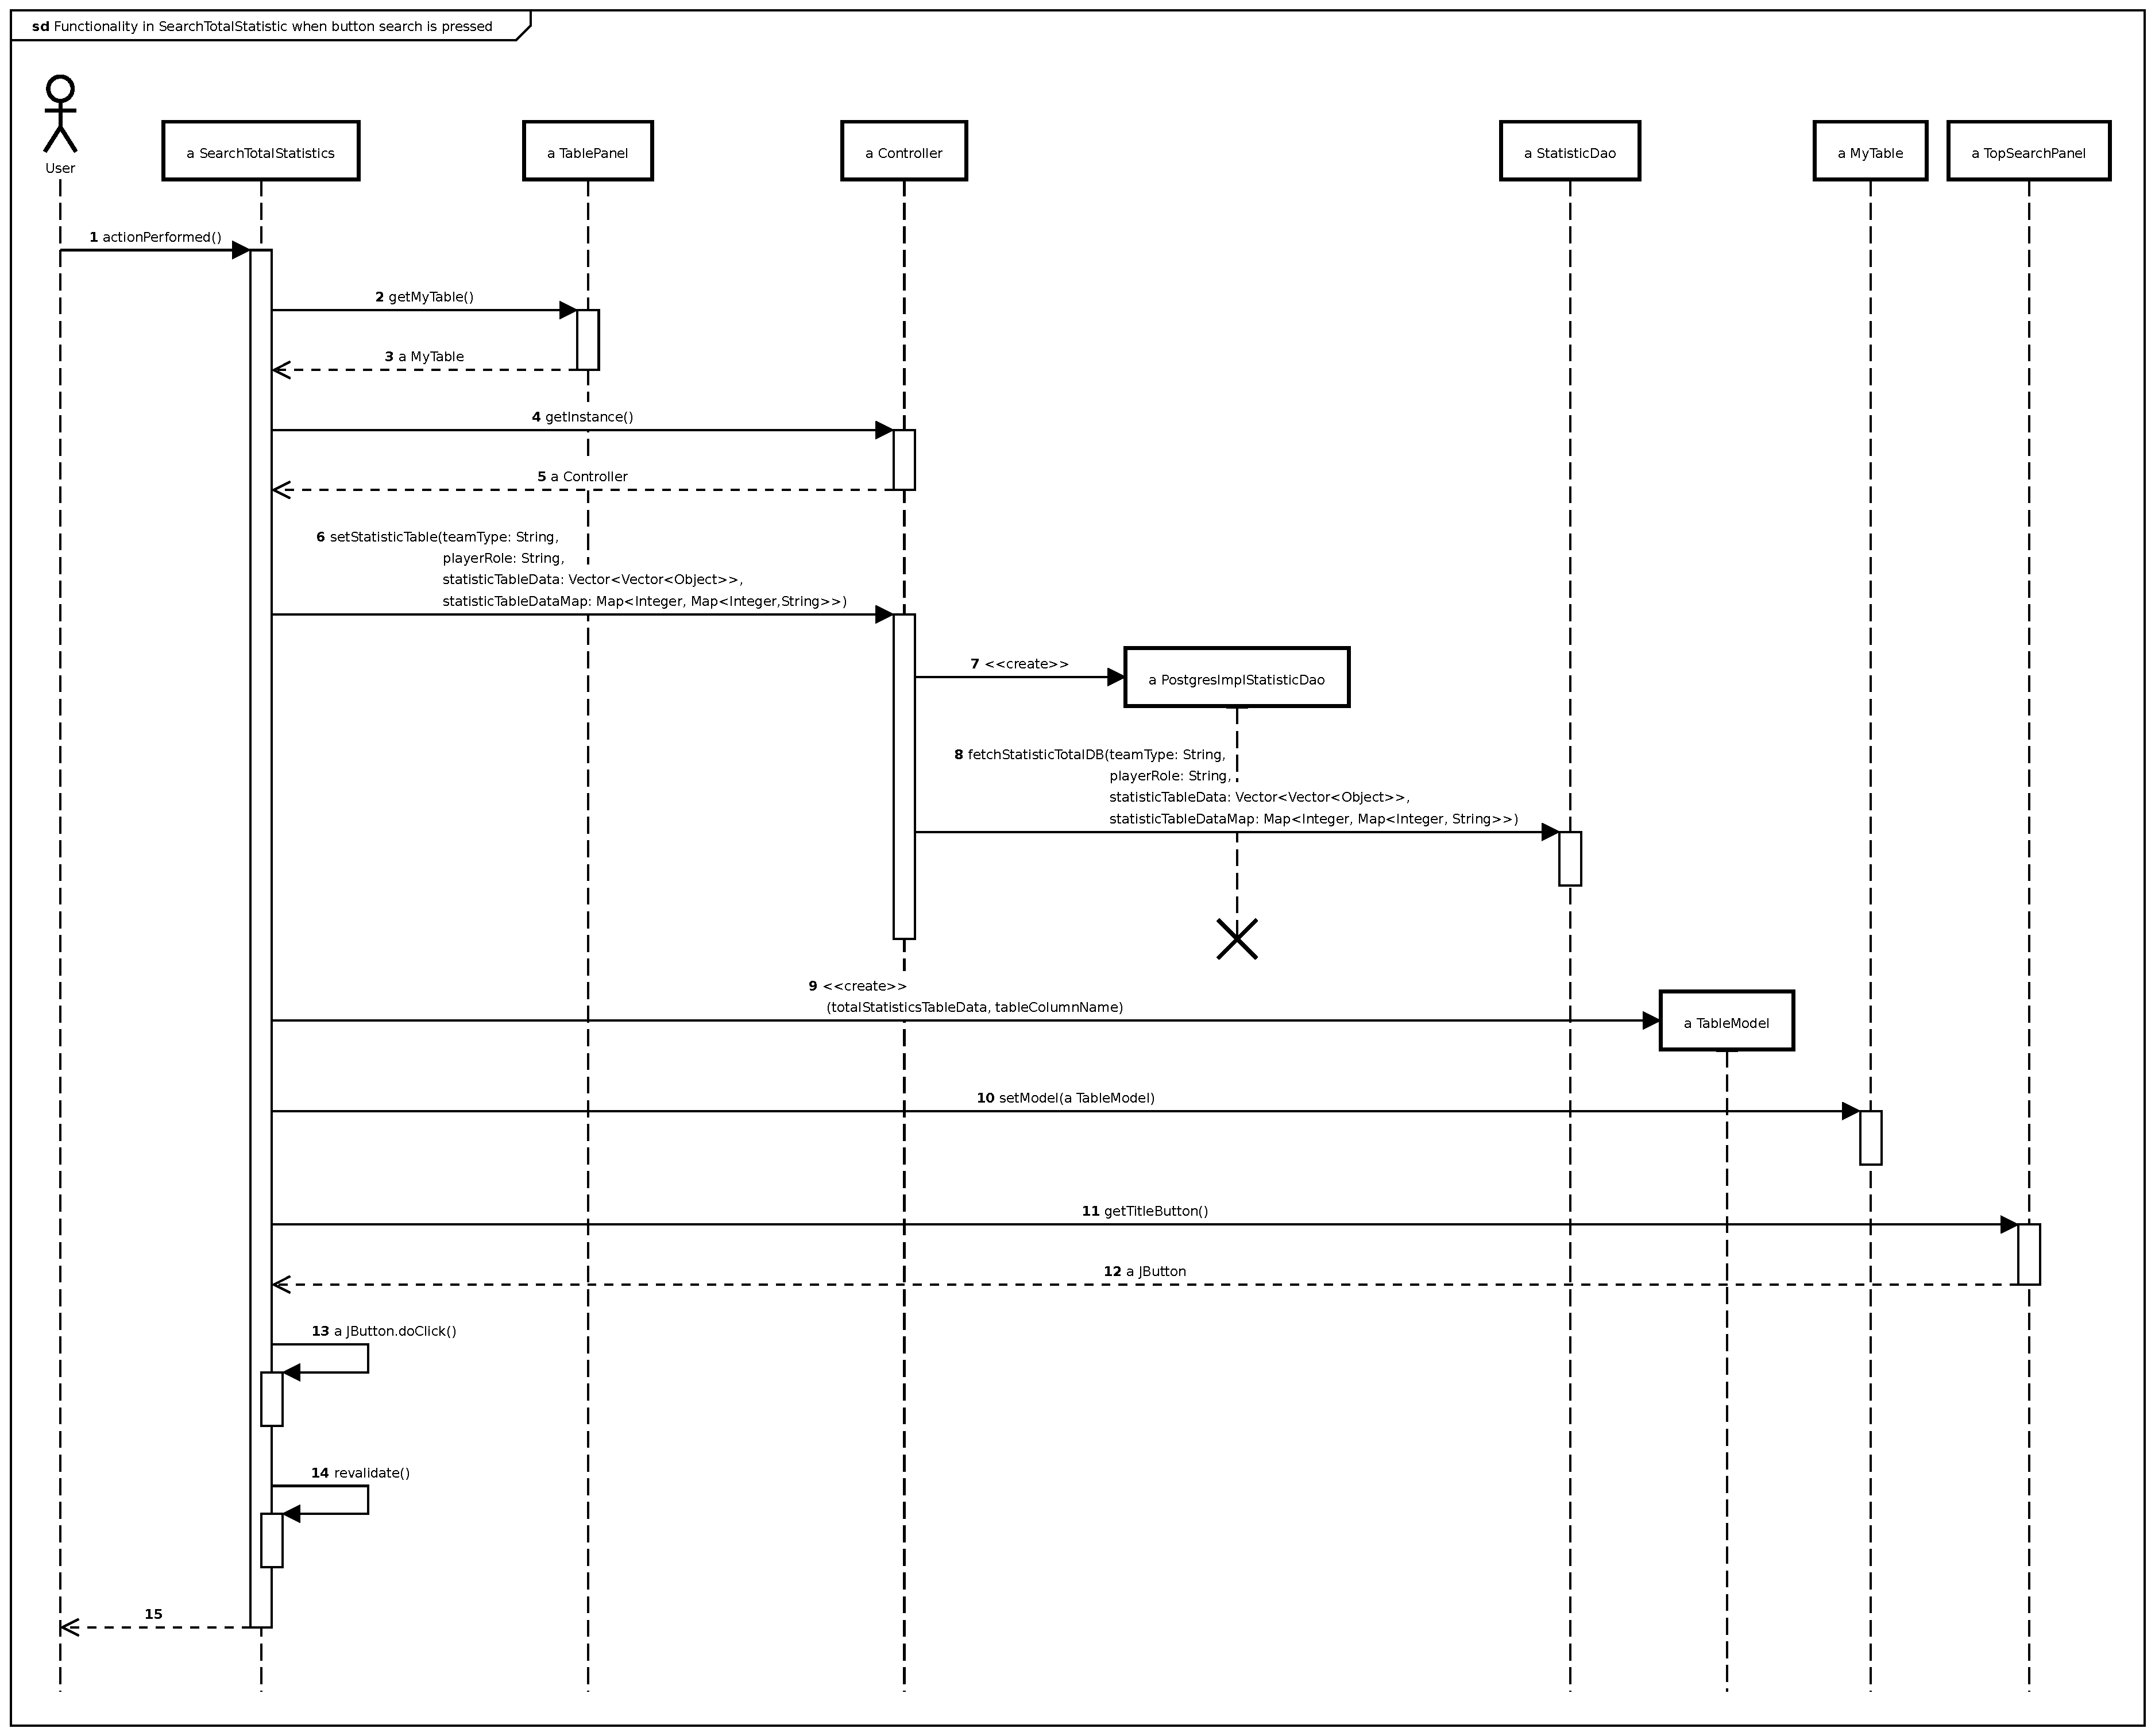
\includepdf[pages=-]{res/DOC_OBJECT/sequenceDiagram1.pdf}
\end{figure}

\newpage

\bigskip
\begin{center}
	\textbf{Sequence Diagram 2}
\end{center}
\bigskip

\begin{figure}[h]
	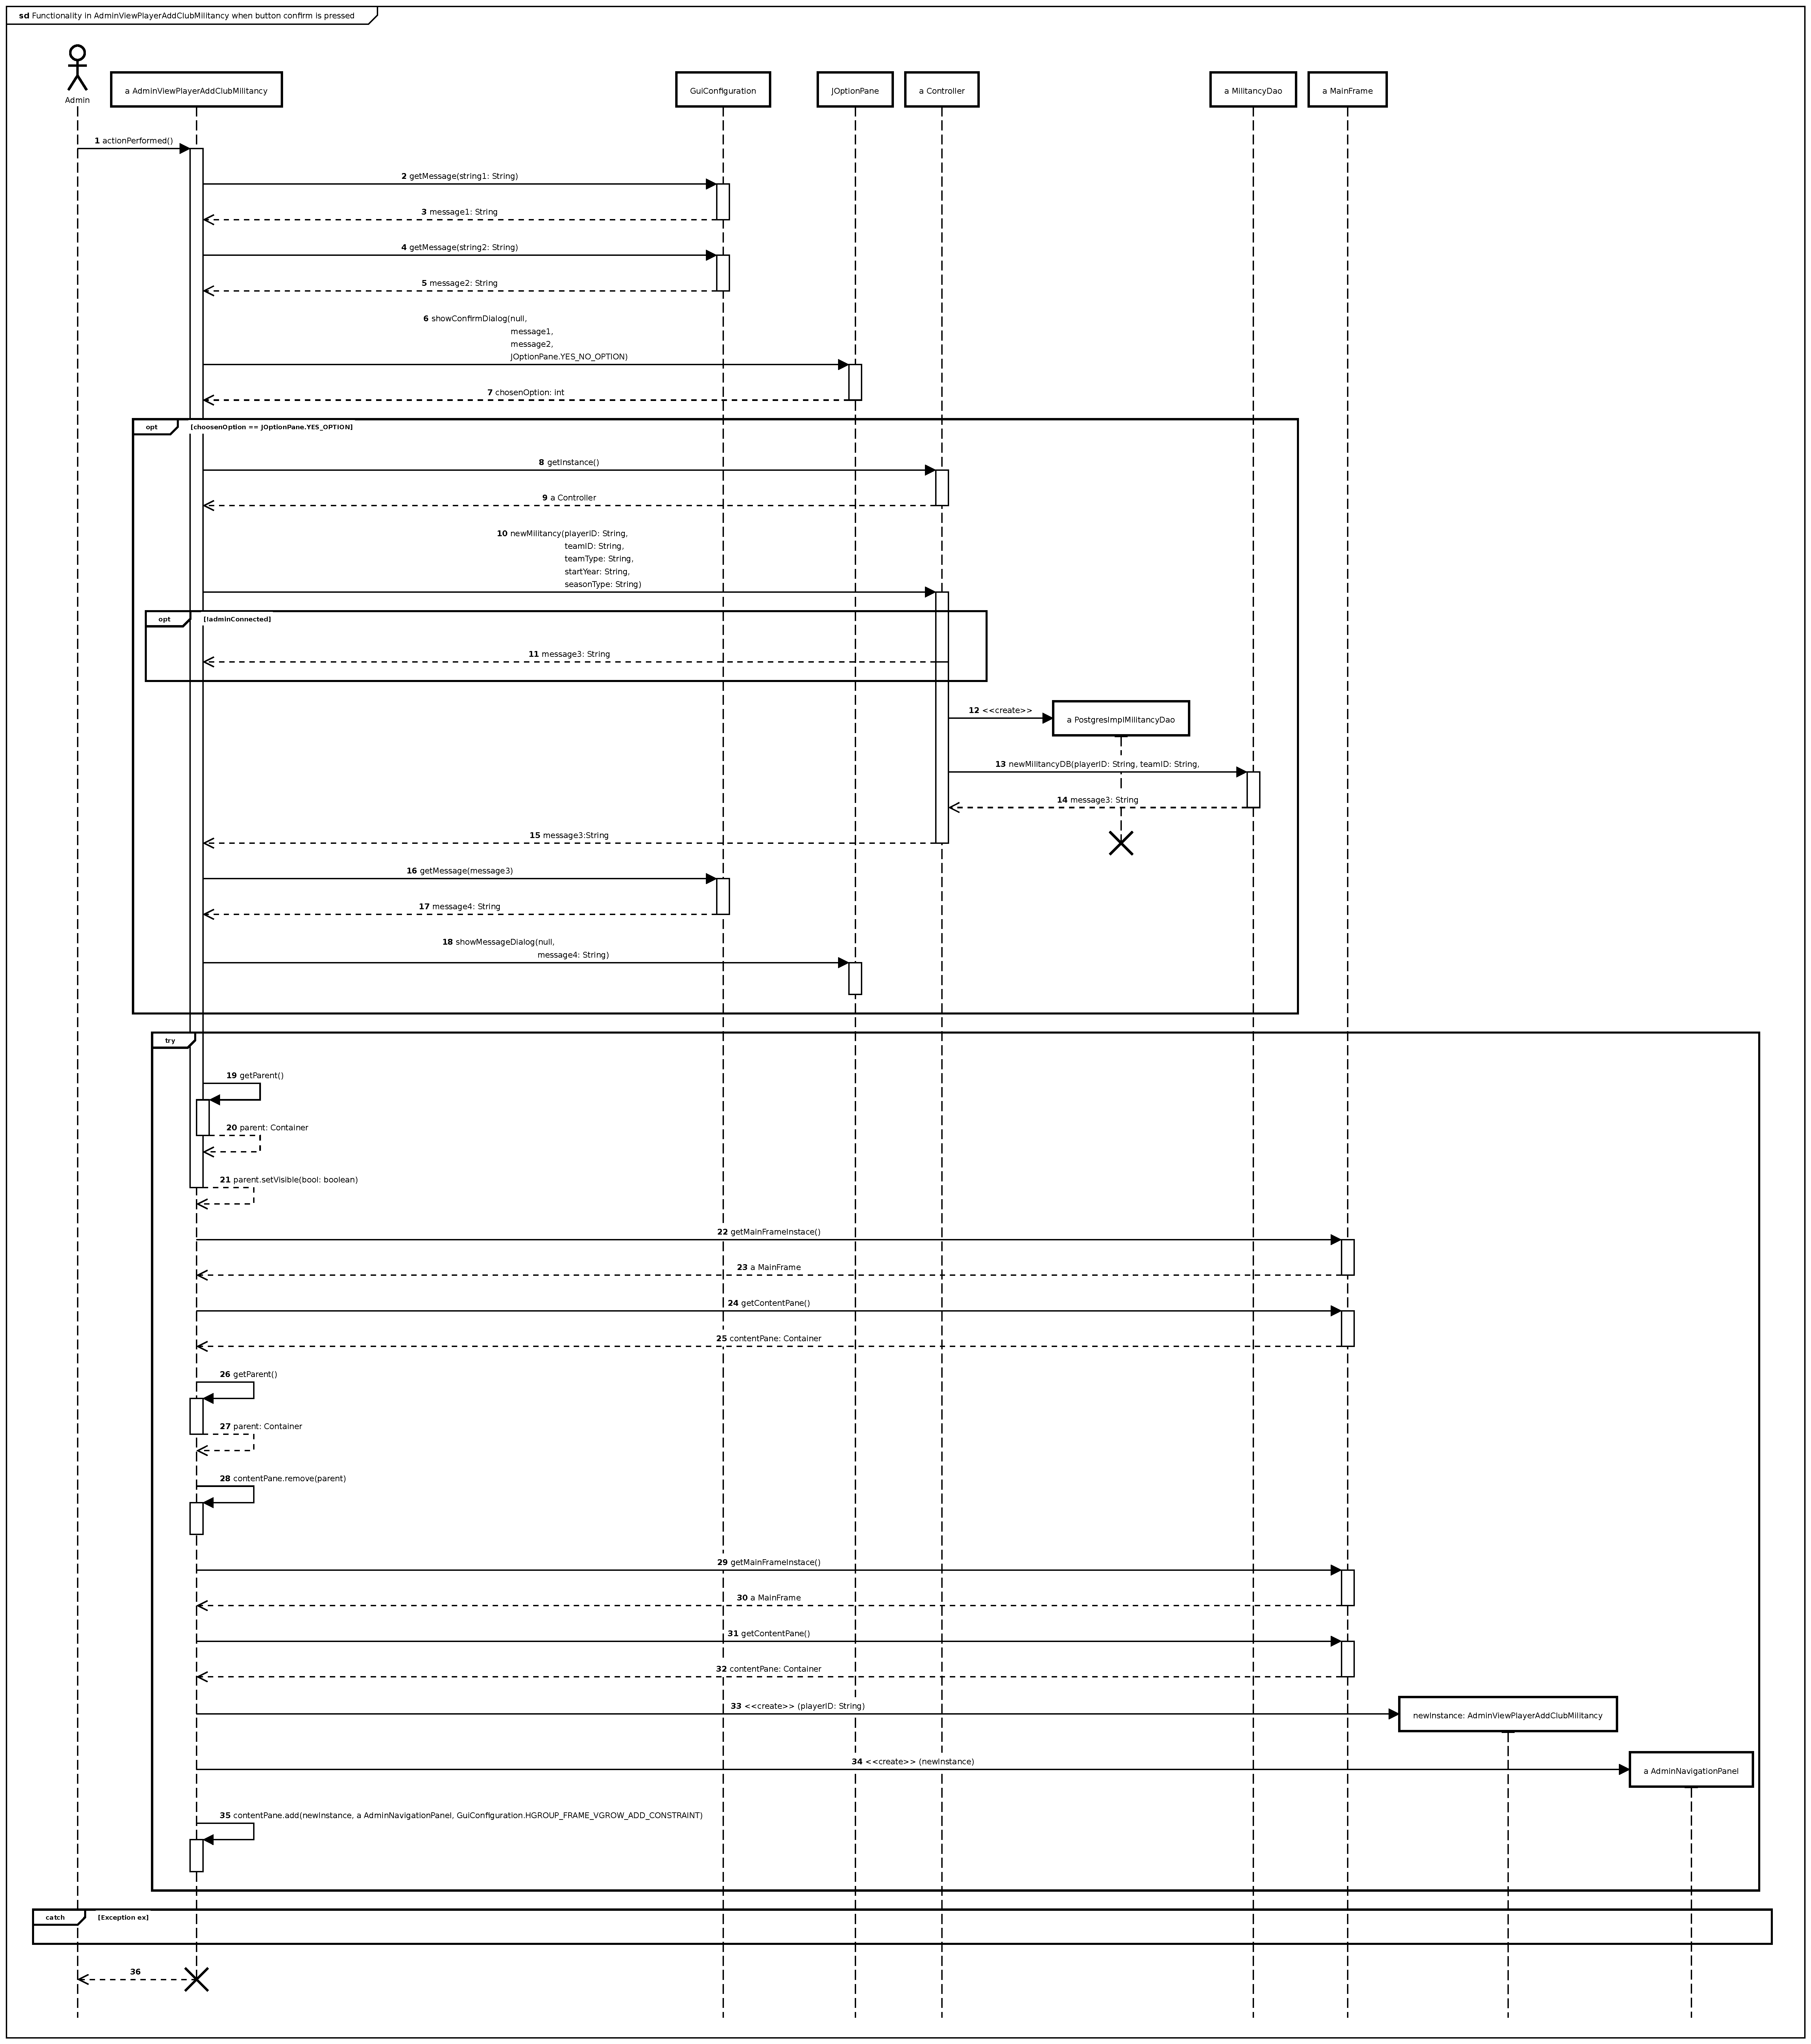
\includepdf[pages=-]{res/DOC_OBJECT/sequenceDiagram2.pdf}
\end{figure}




\end{document}